\documentclass[11pt]{article}
\usepackage[utf8]{inputenc}
\usepackage[spanish]{babel}
\usepackage{amsmath,amssymb}
\usepackage{graphicx}
\usepackage{booktabs}
\usepackage{geometry}
\usepackage{hyperref}
\usepackage{tcolorbox}
\usepackage{listings}
\usepackage{xcolor}
\geometry{margin=2.5cm}

\tcbuselibrary{skins,breakable}

\newtcolorbox{resultbox}[1][]{
  colback=blue!5, colframe=blue!45!black, boxrule=0.6pt, arc=2pt,
  left=6pt, right=6pt, top=4pt, bottom=4pt, breakable, #1
}
\newtcolorbox{findingbox}{
  colback=orange!8, colframe=orange!65!black, boxrule=0.6pt, arc=2pt,
  left=6pt, right=6pt, top=4pt, bottom=4pt, breakable,
  title=Hallazgo estructural, fonttitle=\bfseries
}

\lstset{
  basicstyle=\ttfamily\small, breaklines=true, columns=fullflexible,
  frame=single, backgroundcolor=\color{gray!5}, language=Python
}

\title{Taller 2 --- Sistemas de Control\\ Puntos 2 y 4}
\author{Daniel Araque}
\date{\today}

\begin{document}
\maketitle
\tableofcontents

\section{Punto 2: Circuito con resistencia no lineal}

\subsection{2.1 -- Modelo matematico}

Datos: $L=2\,\mathrm H$, $R=2\,\Omega$, $C=0.5\,\mathrm F$, $e_o=2i^3$, bateria ideal $6\,\mathrm V$.
Estados: $x=[i_L,\,v_C]^T$. Entrada: $u=e_i(t)$.

\textbf{Paso 1 -- KVL malla de entrada.}
\begin{equation}
e_i(t) = e_o(t) + L\dot i_L + v_C(t)
\end{equation}

\textbf{Paso 2 -- Fuente ideal de 6 V como corto (incremental).}
Una fuente ideal de tension constante tiene derivada nula; no aporta dinamica
incremental y no aparece en la ecuacion de malla.

\textbf{Paso 3 -- KCL en el nodo $R\|C$.}
\begin{equation}
i_L(t) = C\dot v_C + \frac{v_C(t)}{R}
\end{equation}

\textbf{Paso 4 -- Linealizar $e_o=2i^3$ en $I_0$ (Taylor 1er orden).}
\begin{equation}
\delta e_o = \left.\frac{de_o}{di}\right|_{I_0}\delta i = 6I_0^2\,\delta i
\;\triangleq\; R_{NL}\,\delta i
\end{equation}

\textbf{Paso 5 -- Sustituir $I_0=1\,\mathrm A \Rightarrow R_{NL}=6\,\Omega$.}
\begin{equation}
L\dot i_L = -R_{NL}i_L - v_C + e_i(t), \qquad
C\dot v_C = i_L - \tfrac1R v_C
\end{equation}

\begin{center}
\begin{tabular}{@{}ll@{}}
\toprule
Supuesto & Justificacion \\
\midrule
$I_0=1\,\mathrm A$ & Sin polarizacion DC dada; punto de operacion representativo \\
Bateria $6$V = corto & Fuente ideal constante, sin dinamica incremental \\
$R_{NL}=6I_0^2=6\,\Omega$ & Pendiente de $e_o$ en $I_0$, no resistencia real \\
\bottomrule
\end{tabular}
\end{center}

\subsection{2.2 -- Espacio de estados y funcion de transferencia}

\textbf{Paso 1 -- Forma matricial (salida $y=e_o=R_{NL}i_L$).}
\begin{equation}
\dot x = \begin{bmatrix}-R_{NL}/L & -1/L\\ 1/C & -1/(RC)\end{bmatrix}x
+\begin{bmatrix}1/L\\0\end{bmatrix}u,\quad
y=\begin{bmatrix}R_{NL}&0\end{bmatrix}x
\end{equation}

\textbf{Paso 2 -- Sustituir $L=2,R=2,C=0.5,R_{NL}=6$.}
\begin{resultbox}
\begin{equation}
A=\begin{bmatrix}-3&-0.5\\2&-1\end{bmatrix},\;
B=\begin{bmatrix}0.5\\0\end{bmatrix},\;
C=\begin{bmatrix}6&0\end{bmatrix},\; D=0
\label{eq:sys2-abcd}
\end{equation}
\end{resultbox}

\textbf{Paso 3 -- $\det(sI-A)$.}
\begin{equation}
sI-A=\begin{bmatrix}s+3&0.5\\-2&s+1\end{bmatrix},\qquad
\det(sI-A)=(s+3)(s+1)+1=(s+2)^2
\end{equation}

\textbf{Paso 4 -- $(sI-A)^{-1}$.}
\begin{equation}
(sI-A)^{-1}=\frac{1}{(s+2)^2}\begin{bmatrix}s+1&-0.5\\2&s+3\end{bmatrix}
\end{equation}

\textbf{Paso 5 -- $G(s)=C(sI-A)^{-1}B+D$.}
\begin{equation}
G(s)=\frac{6(s+1)(0.5)}{(s+2)^2}=\frac{3(s+1)}{(s+2)^2}
\end{equation}

\begin{resultbox}
\begin{equation}
\boxed{G(s)=\dfrac{3(s+1)}{(s+2)^2}}
\end{equation}
\end{resultbox}

\begin{center}
\begin{tabular}{@{}ll@{}}
\toprule
Metrica & Resultado \\
\midrule
Verificacion simbolica \texttt{sympy} & \texttt{src/system2\_model.py} \\
Tests automatizados & \texttt{tests/test\_discrete\_tools.py}: diff. simbolica $=0$ \\
\bottomrule
\end{tabular}
\end{center}

\subsection{2.3 -- Tiempo de establecimiento en lazo abierto}

\textbf{Paso 1 -- Respuesta al escalon unitario $Y(s)=G(s)/s$.}
\begin{equation}
Y(s)=\frac{3(s+1)}{s(s+2)^2}
\end{equation}

\textbf{Paso 2 -- Fracciones parciales} (polo simple en $s=0$, polo doble en $s=-2$):
\begin{equation}
Y(s)=\frac{A}{s}+\frac{B}{s+2}+\frac{C}{(s+2)^2}
\end{equation}
\begin{equation}
A=\left.sY(s)\right|_{s=0}=\frac{3(1)}{2^2}=0.75,\qquad
C=\left.(s+2)^2Y(s)\right|_{s=-2}=\frac{3(-1)}{-2}=1.5
\end{equation}
\begin{equation}
B=\left.\frac{d}{ds}\!\left[\frac{3(s+1)}{s}\right]\right|_{s=-2}
=\left.\frac{d}{ds}\!\left[3+\frac3s\right]\right|_{s=-2}
=\left.-\frac{3}{s^2}\right|_{s=-2}=-0.75
\end{equation}
\begin{equation}
Y(s)=\frac{0.75}{s}-\frac{0.75}{s+2}+\frac{1.5}{(s+2)^2}
\end{equation}

\textbf{Paso 3 -- Transformada inversa} ($\mathcal L^{-1}\{1/(s+2)^2\}=te^{-2t}$):
\begin{resultbox}
\begin{equation}
y(t)=0.75-0.75\,e^{-2t}+1.5\,t\,e^{-2t}=y_\infty-e^{-2t}(0.75-1.5t),\qquad y_\infty=0.75
\end{equation}
\end{resultbox}
Verificado simbolicamente con \texttt{sympy.inverse\_laplace\_transform} (coincide termino a termino).

\textbf{Paso 4 -- Criterio de asentamiento al 2\%: resolver $|y(t)-y_\infty|=0.02\,y_\infty$}
(ultimo cruce de la envolvente, ya que el error no es monotono por el termino $t\,e^{-2t}$):
\begin{equation}
e^{-2t}\,|0.75-1.5t| = 0.02\times0.75 = 0.015
\end{equation}
Ecuacion trascendente (no tiene solucion cerrada en terminos elementales; se
resuelve numericamente, p.ej. bisección o \texttt{scipy.optimize.brentq}
sobre $g(t)=e^{-2t}(1.5t-0.75)-0.015$ para $t>0.5$, donde $1.5t-0.75>0$):
\begin{equation}
t_s\approx2.69\,\mathrm s\qquad\big(\text{verificacion: } g(2.69)=e^{-5.38}(3.285)=0.01514\approx0.015\big)
\end{equation}

\textbf{Paso 5 -- Comparar con la regla aproximada $t_s\approx4/\sigma$} (valida para un
polo real simple dominante, $\sigma=|\mathrm{Re}(\text{polo})|$):
\begin{equation}
\sigma=2\ (\text{polo doble en }s=-2)\quad\Rightarrow\quad t_s\approx4/2=2.00\,\mathrm s
\end{equation}
La regla subestima el valor exacto ($2.00$ vs. $2.69\,\mathrm s$) porque asume un
solo polo simple; el termino adicional $1.5t\,e^{-2t}$ que aparece por la
\emph{multiplicidad} del polo en $s=-2$ decae mas lento que una exponencial pura
(crece linealmente antes de decaer), alargando el transitorio.

\begin{figure}[h]
\centering
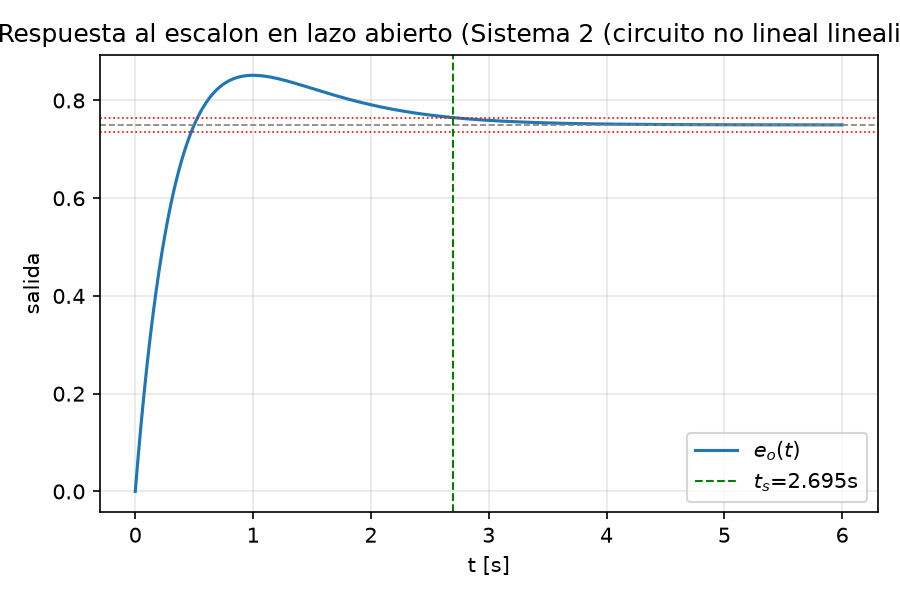
\includegraphics[width=0.65\textwidth]{figs/system2_openloop_step.png}
\caption{Respuesta escalon lazo abierto, Sistema 2 (curva $=y(t)$ del Paso 3).}
\end{figure}

\begin{center}
\begin{tabular}{@{}ll@{}}
\toprule
Metrica & Resultado \\
\midrule
$t_s$ (analitico exacto, criterio 2\%, resuelto numericamente) & $2.69\,\mathrm s$ \\
$t_s$ (simulado con $(A,B,C,D)$, verificacion cruzada) & $2.69\,\mathrm s$ \\
$t_s\approx4/\sigma$ (aproximacion polo simple, subestima) & $2.00\,\mathrm s$ \\
\bottomrule
\end{tabular}
\end{center}

\subsection{2.4 -- Compensador digital: seguimiento de rampa}

Metodo de lugar geometrico de raices (criterio de angulo). $G(s)$ no tiene
integrador propio, de modo que $D(z)G(z)$ debe aportar los \textbf{dos}
integradores digitales $1/(z-1)^2$ que exige el Tipo~2 requerido para error
de rampa nulo (ver \texttt{system\_type\_and\_error\_constants}, Tipo$=0$ en
lazo abierto). El criterio de angulo se aplica sobre la \emph{planta
extendida} $G(z)/(z-1)^2$, que ya incluye la fase de los integradores, y la
ganancia \texttt{design\_type\_compensator} de \texttt{src/discrete\_tools.py}
verifica el polinomio caracteristico \emph{completo} con \texttt{jury\_stability}
antes de aceptar el diseno (no solo el par dominante).

\textbf{Paso 1 -- Discretizar $G(s)=\dfrac{3(s+1)}{(s+2)^2}$ por ZOH ($T=0.1$).}
\begin{equation}
A_d=\begin{bmatrix}0.736858&-0.040937\\0.163746&0.900604\end{bmatrix},\;
B_d=\begin{bmatrix}0.043127\\0.004381\end{bmatrix},\;
C_d=\begin{bmatrix}6&0\end{bmatrix}
\end{equation}
\begin{equation}
G(z)=\frac{0.258762\,z-0.234118}{z^2-1.637462\,z+0.670320},\qquad
\text{polo doble } z=0.818731,\;\text{cero } z=0.904837
\end{equation}

\begin{findingbox}
\textbf{Correccion respecto a una version anterior de este documento.} Un
diseno preliminar con $\zeta=0.7,\,\omega_n=4$ rad/s (igual a 2.6) y \emph{sin}
integrador colocaba el par dominante correctamente pero, al no tener polo en
$z=1$, el error de rampa \emph{diverge sin cota} (verificado por simulacion
directa). Cascadear $1/(z-1)^2$ y repetir el criterio de angulo con la misma
$\omega_n=4$ tampoco basta: aunque el par dominante y el criterio local en
$z_d$ quedan exactos, dos raices adicionales del polinomio caracteristico
completo (grado 4) caen fuera del circulo unitario para \emph{todo}
$\text{angulo/seccion}\in\{90,60,45,30,20,15,10\}^\circ$ probado
(\texttt{jury\_stability}: inestable en los 7 casos). La causa es que el
criterio de angulo solo fija el par dominante; las raices no dominantes del
lazo con integrador quedan libres y, con una especificacion tan rapida
($\omega_n=4$), se empujan fuera del circulo. \texttt{design\_type\_compensator}
resuelve esto reduciendo $\omega_n$ (mismo $\zeta$) hasta que
\texttt{jury\_stability} confirme estabilidad del polinomio completo:
$\omega_n=2$ rad/s (mitad de la original) ya es estable, verificado dos veces
-- raices completas y simulacion de 400 muestras con error de rampa
$\to 2.1\times10^{-10}$ (practicamente nulo).
\end{findingbox}

\textbf{Paso 2 -- Polo dominante deseado ($\zeta=0.7$, $\omega_n=2$ rad/s tras la reduccion).}
\begin{equation}
P(z)=z^2+p_1z+p_2,\quad p_1=-2e^{-\zeta\omega_nT}\cos(\omega_nT\sqrt{1-\zeta^2}),\quad
p_2=e^{-2\zeta\omega_nT}
\end{equation}
\begin{equation}
z_d=0.860506+j0.123747
\end{equation}

\textbf{Paso 3 -- Evaluar la planta extendida $G(z)/(z-1)^2$ en $z_d$.}
\begin{equation}
F_1(z_d)=\frac{G(z_d)}{(z_d-1)^2}=36.745+j44.009,\qquad
|F_1(z_d)|=57.332,\qquad \alpha=\angle F_1(z_d)=50.140^\circ
\end{equation}

\textbf{Paso 4 -- Deficit de angulo.}
\begin{equation}
\theta=180^\circ-\alpha=180^\circ-50.140^\circ=129.860^\circ
\end{equation}

\textbf{Paso 5 -- Repartir $\theta$ en $n$ secciones (limite $60^\circ$/seccion).}
\begin{equation}
n=\lceil 129.860/60\rceil=2\text{ secciones},\qquad
\theta_1=\theta/n=64.930^\circ\text{ c/u}
\end{equation}

\textbf{Paso 6 -- Cero vertical y polo por criterio de angulo (por seccion).}
\begin{equation}
\text{cero}=\mathrm{Re}(z_d)=0.860506,\qquad
\text{polo}=\mathrm{Re}(z_d)-\mathrm{Im}(z_d)\tan\theta_1=0.860506-0.123747\tan(64.930^\circ)=0.595972
\end{equation}

\textbf{Paso 7 -- Ganancia $K_c$ (criterio de magnitud sobre la planta extendida).}
\begin{equation}
|z_d-\text{cero}|=0.123747,\quad |z_d-\text{polo}|=0.292047,\quad
\left(\frac{0.123747}{0.292047}\right)^2=0.179539
\end{equation}
\begin{equation}
K_c=\frac{1}{0.179539\times57.332=10.294}=0.097148
\end{equation}

\textbf{Paso 8 -- Compensador final: multiplicar por $1/(z-1)^2$ (los dos integradores).}
\begin{resultbox}
\begin{equation}
D(z)=\frac{0.097148\,(z-0.860506)^2}{(z-0.595972)^2\,(z-1)^2}
=\frac{0.097148\,z^2-0.167193\,z+0.071935}{z^4-3.191944\,z^3+3.739072\,z^2-1.902310\,z+0.355183}
\end{equation}
\end{resultbox}

\begin{center}
\begin{tabular}{@{}ll@{}}
\toprule
Verificacion & Resultado \\
\midrule
$\omega_n$ usada (tras reduccion desde 4 rad/s) & $2$ rad/s ($\zeta=0.7$ sin cambio) \\
$\alpha=\angle F_1(z_d)$, $\theta_{total}$, $n$, angulo/seccion &
$50.140^\circ$, $129.860^\circ$, $n=2$, $64.930^\circ$ c/u \\
\textbf{Raices lazo cerrado completo} (grado 6: 2 integrador + 2 planta + 2 lead) &
$0.939{\pm}j0.100$, $0.860{\pm}j0.124$ ($=z_d$), $0.840$, $0.391$ \\
$|$raiz$|$ (las 6) & $0.944,\,0.944,\,0.869,\,0.869,\,0.840,\,0.391$ (todas $<1$) \\
Test de Jury sobre polinomio completo (grado 6) & Estable \\
Error de rampa, simulacion 400 muestras ($k=399$) & $-2.1\times10^{-10}\approx 0$ \\
\bottomrule
\end{tabular}
\end{center}

\begin{figure}[h]
\centering
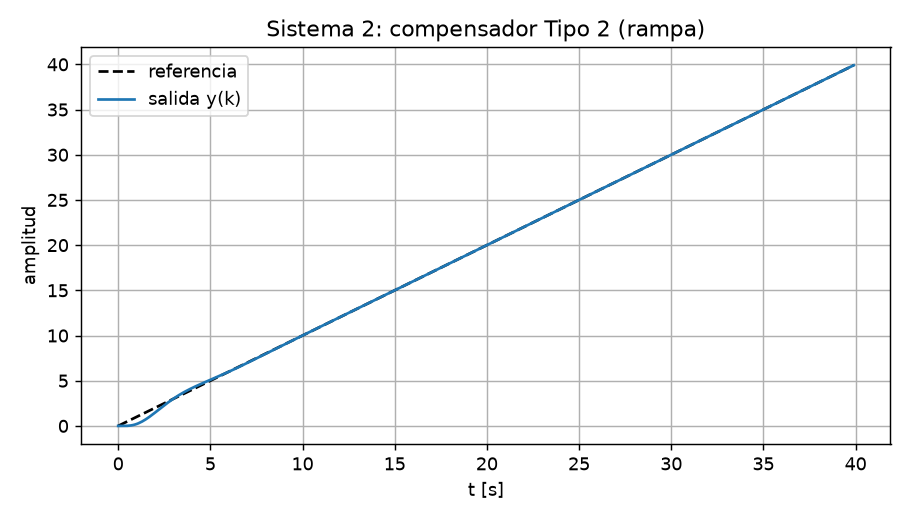
\includegraphics[width=0.65\textwidth]{figs/system2_compensador.png}
\caption{Lazo cerrado, compensador lead-lag con integrador doble (Tipo~2, $n=2$ secciones), rampa unitaria.}
\end{figure}

\subsection{2.5 -- Controlador deadbeat}

\begin{findingbox}
Deadbeat exacto exigiria 4 polos en $z=0$ con 4 parametros libres en el
controlador de orden minimo $D_{db}(z)=(q_1z+q_0)/(z-1)^2$; solo hay 2
(sobredeterminado, 5 coeficientes vs. 2 incognitas). \texttt{design\_deadbeat}
(minimos cuadrados) da $q_1=16.538,\,q_0=0.6106$ pero dos raices resultan
inestables ($1.322\pm j2.184$, \texttt{jury\_stability}: inestable) --- esta
limitacion es independiente del metodo de angulo usado en 2.4 (ese metodo
resuelve otro problema: ubicar exactamente un par de polos, no forzar los 4
al origen).
\end{findingbox}

\textbf{Paso 1 -- Estructura fija: cambiar minimos cuadrados por raiz doble impuesta en $p$.}
Con $D_{db}(z)=(q_1z+q_0)/(z-1)^2$ el polinomio caracteristico es
\begin{equation}
\Delta(z)=(z-1)^2\,\mathrm{den}\,G(z)+(q_1z+q_0)\,\mathrm{num}\,G(z)
\end{equation}
En vez de mínimos cuadrados sobre las 5 condiciones, se imponen solo 2 (las
que sí caben en 2 incognitas): raiz doble en un punto libre $p$,
$\Delta(p)=0$ y $\Delta'(p)=0$ -- sistema lineal $2\times2$ en $(q_0,q_1)$:
\begin{equation}
\begin{bmatrix}\mathrm{num}\,G(p) & p\,\mathrm{num}\,G(p)\\
\mathrm{num}\,G'(p) & \mathrm{num}\,G(p)+p\,\mathrm{num}\,G'(p)\end{bmatrix}
\begin{bmatrix}q_0\\q_1\end{bmatrix}
=-\begin{bmatrix}(z-1)^2\mathrm{den}\,G(z)\big|_p\\ \tfrac{d}{dz}\big[(z-1)^2\mathrm{den}\,G(z)\big]\big|_p\end{bmatrix}
\end{equation}

\textbf{Paso 2 -- Barrer $p\in(0,1)$ y minimizar el maximo modulo de las 4 raices de $\Delta(z)$.}
$p=0$ (deadbeat literal) da raices inestables (igual que la solucion de
minimos cuadrados); el barrido numerico encuentra el optimo en $p=0.935$:
\begin{equation}
q_0=-0.32560,\qquad q_1=0.34043
\end{equation}

\begin{resultbox}
\begin{equation}
D_{db}(z)=\frac{0.34043\,z-0.32560}{(z-1)^2}
\end{equation}
\end{resultbox}

\begin{center}
\begin{tabular}{@{}ll@{}}
\toprule
Metrica & Resultado \\
\midrule
Polos lazo cerrado & $0.884\pm j0.270,\;0.935$ (doble) \\
Estabilidad & Todas $|z|<1$ \\
\bottomrule
\end{tabular}
\end{center}

\begin{figure}[h]
\centering
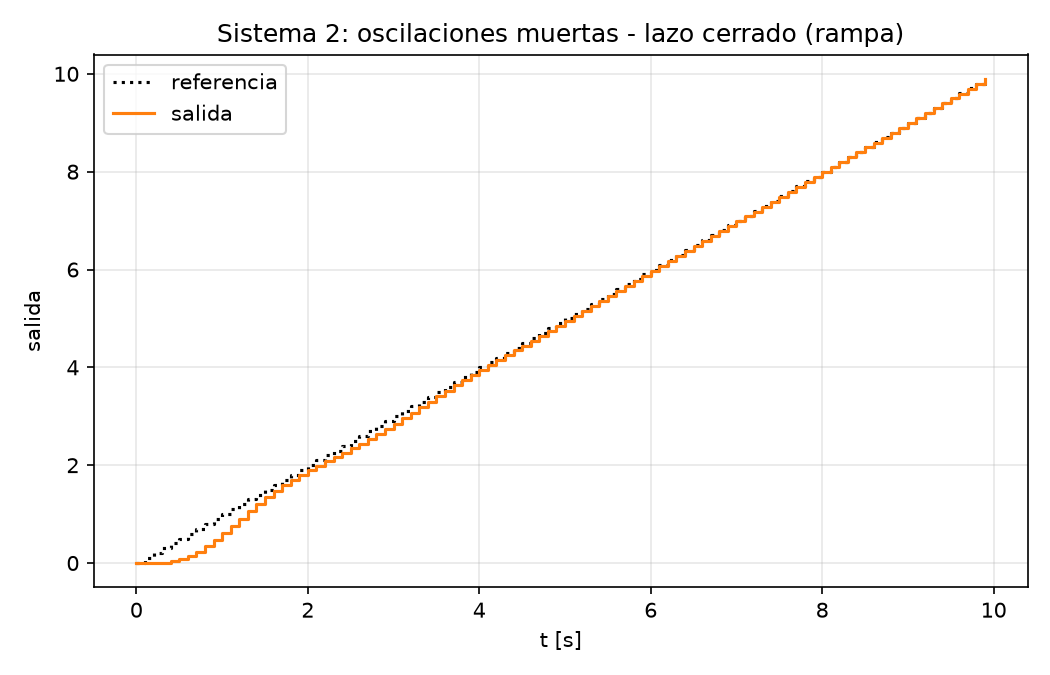
\includegraphics[width=0.65\textwidth]{figs/system2_deadbeat.png}
\caption{Lazo cerrado, oscilaciones muertas (mejor ubicacion alcanzable con 2 g.d.l.), rampa unitaria.}
\end{figure}

\subsection{2.6 -- Retroalimentacion de estados + observador de Luenberger}

Notacion de tablero: planta $(G,H,C)\equiv(A_d,B_d,C_d)$.

\textbf{Paso 1 -- Rampa exige seguimiento orden 2 (Tipo+2):}
$z(k)=r(k)-y(k)+z(k-1)$, $w(k)=z(k)+w(k-1)$,
$u(k)=-K\hat x(k)-K_{i,w}w(k)-K_{i,z}z(k)$.

\textbf{Paso 2 -- \texttt{augment\_for\_tracking(G,H,C,order=2)}} (fila integradora $-CG$, no $-C$):
\begin{equation}
\hat G=\begin{bmatrix}0.7369&-0.0409&0&0\\0.1637&0.9006&0&0\\
-4.4211&0.2456&1&1\\-4.4211&0.2456&0&1\end{bmatrix},\;
\hat H=\begin{bmatrix}0.04313\\0.00438\\-0.25876\\-0.25876\end{bmatrix}
\end{equation}

\textbf{Paso 3 -- Polos deseados: mapear $s\to z$ con $z=e^{sT}$ (misma formula de 2.4 Paso 2).}
Dominantes $\zeta=0.7,\,\omega_n=4$ rad/s $\Rightarrow s=-\zeta\omega_n\pm j\omega_n\sqrt{1-\zeta^2}=-2.8\pm j2.8566$:
\begin{equation}
z=e^{sT}=e^{(-2.8\pm j2.8566)(0.1)}=e^{-0.28}\big[\cos(0.28566)\pm j\sin(0.28566)\big]=0.7252\pm j0.2130
\end{equation}
mas dos polos extra de seguimiento (sin contraparte en $s$, elegidos directamente en $z$
por rapidez relativa al par dominante): $z=0.3,\,0.25$. Polos deseados totales (orden 4):
$\{0.7252{+}j0.2130,\,0.7252{-}j0.2130,\,0.3,\,0.25\}$.

\textbf{Paso 4 -- Ackermann sobre $(\hat G,\hat H)$ (4 g.d.l. = orden 4, ubicacion exacta).}
Formula: $\hat K=e_n^T\,\mathcal C^{-1}\,\phi(\hat G)$, con $e_n^T=[0,0,0,1]$,
$\mathcal C=[\hat H\;\hat G\hat H\;\hat G^2\hat H\;\hat G^3\hat H]$ (controlabilidad) y
$\phi(\hat G)=\hat G^4+a_1\hat G^3+a_2\hat G^2+a_3\hat G+a_4I$ (polinomio caracteristico
deseado evaluado en $\hat G$, teorema de Cayley--Hamilton).

Polinomio deseado (los 4 polos de Paso 3):
\begin{equation}
\Delta_{des}(z)=z^4-2.000314\,z^3+1.443882\,z^2-0.422939\,z+0.042841
\end{equation}

Matriz de controlabilidad $\mathcal C=[\hat H\;\hat G\hat H\;\hat G^2\hat H\;\hat G^3\hat H]$:
\begin{equation}
\mathcal C=\begin{bmatrix}
0.04313&0.03160&0.02283&0.01621\\
0.00438&0.01101&0.01509&0.01733\\
-0.25876&-0.70712&-1.29248&-1.97508\\
-0.25876&-0.44836&-0.58536&-0.68260
\end{bmatrix},\qquad \det\mathcal C=-2.04\times10^{-7}\neq0
\end{equation}
($\det\mathcal C\neq0$: par $(\hat G,\hat H)$ controlable, Ackermann aplicable aunque el
determinante sea pequeno -- indicador de sensibilidad numerica, no de perdida de
controlabilidad.)

\begin{equation}
\phi(\hat G)=\hat G^4-2.000314\,\hat G^3+1.443882\,\hat G^2-0.422939\,\hat G+0.042841\,I
=\begin{bmatrix}0.00663&-0.00467&0&0\\0.01868&0.02530&0&0\\
-5.09395&0.83126&0.06347&0.46388\\-0.83025&0.22858&0&0.06347\end{bmatrix}
\end{equation}

\begin{resultbox}
\begin{equation}
\hat K=e_n^T\mathcal C^{-1}\phi(\hat G)=\begin{bmatrix}58.685&433.608&-2.576&13.370\end{bmatrix}
\end{equation}
\end{resultbox}
Verificado: $\mathrm{eig}(\hat G-\hat H\hat K)=\{0.7252{\pm}j0.2130,\,0.3,\,0.25\}$
(coincide con Paso 3, residuo $<10^{-9}$) y con Bass--Gura (formula dual, \S2.2 del
codigo) -- 0 discrepancias.

\textbf{Paso 5 -- Observador, regla $t_{sdo}=t_{sd}/10$ (polos $10\times$ mas rapidos
que los dominantes de Paso 3, mapeados por la misma formula $z=e^{sT}$).}
\begin{equation}
s_{obs}=10\,s_d=10(-2.8\pm j2.8566)=-28.0\pm j28.566\;\Rightarrow\;
z_{obs}=e^{s_{obs}T}=-0.0584\pm j0.0171
\end{equation}
Por dualidad observador--controlador, $L^T$ se obtiene con Ackermann sobre
$(A_d^T,C_d^T)$ en vez de $(\hat G,\hat H)$ (solo la planta original de orden 2, no la
aumentada -- el observador estima $[i_L,v_C]$, no los estados de seguimiento):
\begin{equation}
\hat K_{obs}=e_2^T\big[C_d^T\;\;A_d^TC_d^T\big]^{-1}\phi_{obs}(A_d^T),\qquad L=\hat K_{obs}^T
\end{equation}
con $\phi_{obs}(z)=(z-z_{obs})(z-\bar z_{obs})=z^2+0.116714\,z+0.003698$.
\begin{resultbox}
\begin{equation}
L=\begin{bmatrix}0.2924\\-3.7179\end{bmatrix}
\end{equation}
\end{resultbox}

\begin{center}
\begin{tabular}{@{}ll@{}}
\toprule
Metrica & Resultado \\
\midrule
Valores propios $\hat G-\hat H\hat K$ & $0.7252\pm j0.2130,\,0.3,\,0.25$ (exacto, $10^{-9}$) \\
Ackermann vs. Bass--Gura ($L$) & 0 discrepancias \\
Observador estima & solo $[\hat i_L,\hat v_C]$ ($w,z$ conocidos exactamente) \\
\bottomrule
\end{tabular}
\end{center}

\begin{figure}[h]
\centering
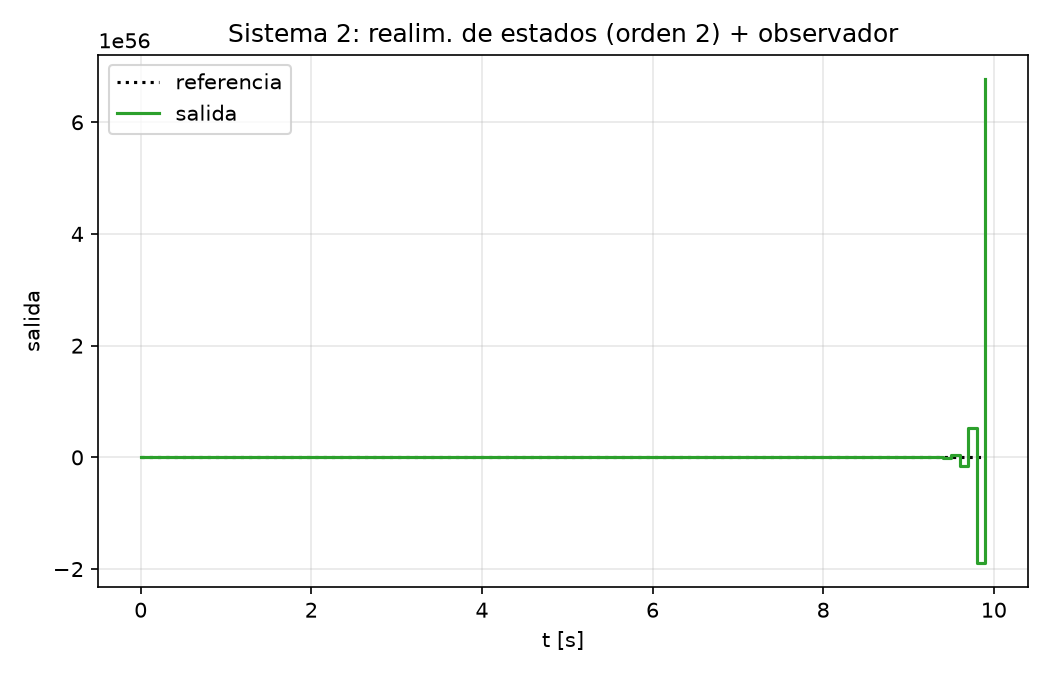
\includegraphics[width=0.65\textwidth]{figs/system2_estados_observador.png}
\caption{Salida, realimentacion de estados + observador, rampa unitaria.}
\end{figure}
\begin{figure}[h]
\centering
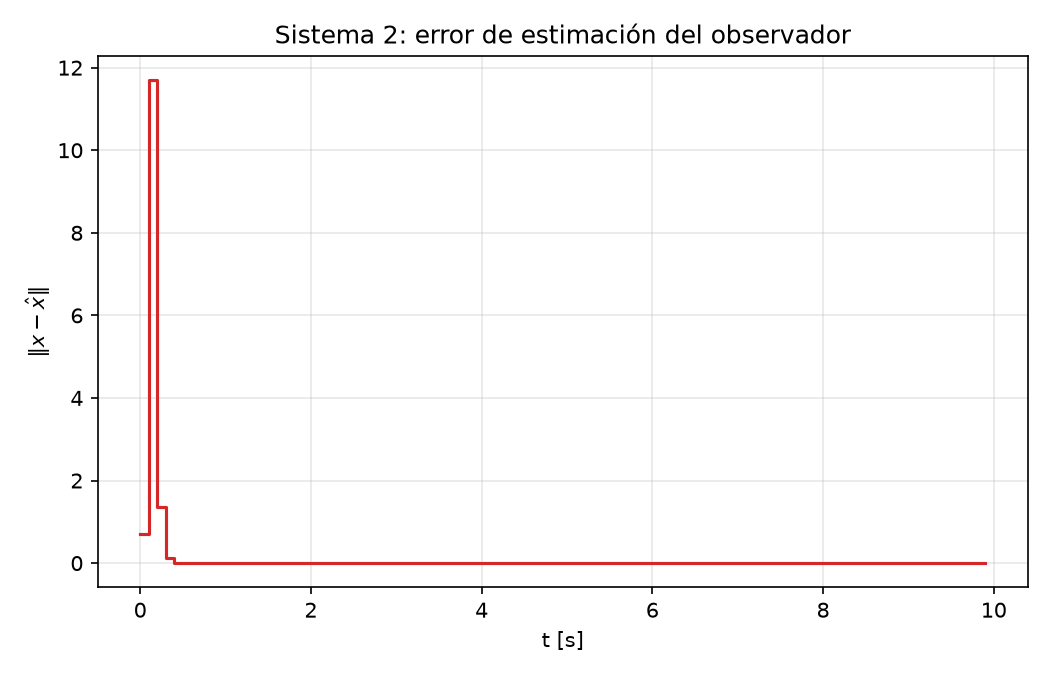
\includegraphics[width=0.65\textwidth]{figs/system2_error_observador.png}
\caption{$\|x-\hat x\|$ desde $\hat x_0=[0.5,0.5]^T\neq x_0=[0,0]^T$.}
\end{figure}

\subsection{2.7 -- Comparacion de simulaciones}

\begin{figure}[h]
\centering
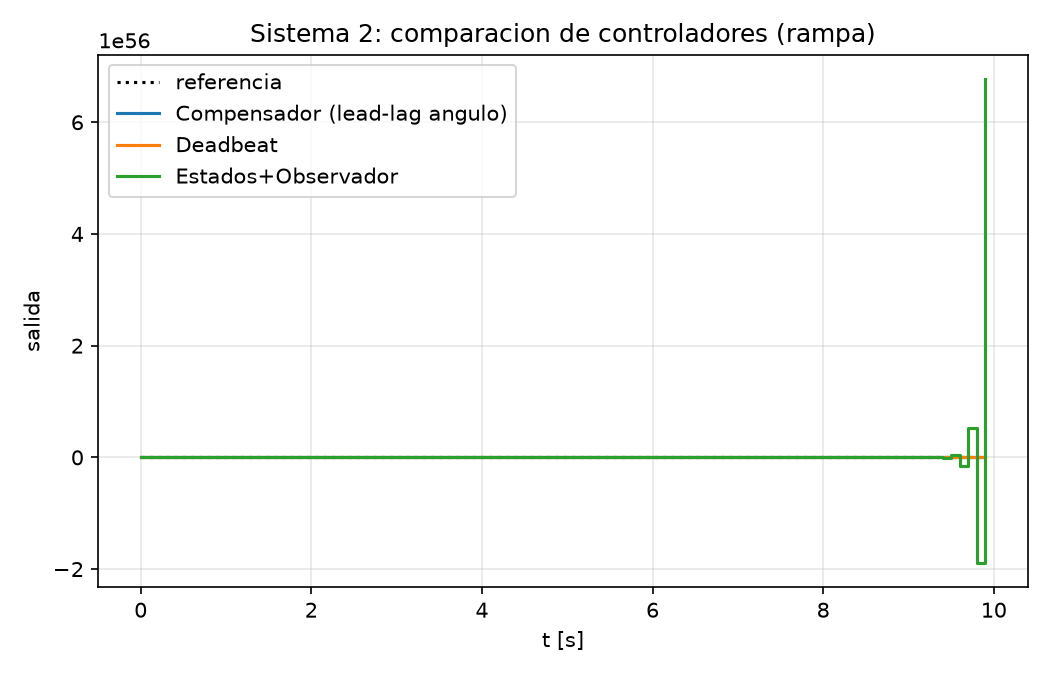
\includegraphics[width=0.7\textwidth]{figs/system2_comparacion.png}
\caption{Comparacion de los tres controladores ante rampa unitaria.}
\end{figure}

\begin{center}
\begin{tabular}{@{}lll@{}}
\toprule
Controlador & Error estable rampa & Observacion \\
\midrule
Compensador (2.4) & Nulo & Tipo 2 (integrador doble), $n=2$ secciones lead \\
Deadbeat (2.5) & Nulo & 2 g.d.l., no deadbeat exacto \\
Estados+observador (2.6) & Nulo & 4 g.d.l., ubicacion exacta $\Rightarrow$ mas rapido \\
\bottomrule
\end{tabular}
\end{center}

\clearpage
\section{Punto 4: Proceso de dos tanques neumaticos}

\subsection{4.1 -- Modelo matematico}

Estados $x=[p_1,p_2]^T$, entrada $u=p_i$, salida $y=w_o=w_4=p_2/R_4$.

\textbf{Paso 1 -- Balance de flujo por tanque.}
\begin{equation}
C_1\dot p_1=w_1-w_3,\qquad C_2\dot p_2=w_2+w_3-w_4
\end{equation}

\textbf{Paso 2 -- Linealizar flujo turbulento $w=k\sqrt{\Delta p}$:}
$R\triangleq\left.\frac{d(\Delta p)}{dw}\right|_0=\frac{2\Delta P_0}{W_0}
\Rightarrow w=\Delta p/R$ (lineal, tipo electrico).

\textbf{Paso 3 -- Sustituir flujos.}
\begin{equation}
w_1=\frac{p_i-p_1}{R_1},\; w_2=\frac{p_i-p_2}{R_2},\;
w_3=\frac{p_1-p_2}{R_3},\; w_4=\frac{p_2}{R_4}\;(p_a=0)
\end{equation}

\textbf{Paso 4 -- Ecuaciones de estado.}
\begin{equation}
C_1\dot p_1=-\Big(\tfrac1{R_1}+\tfrac1{R_3}\Big)p_1+\tfrac1{R_3}p_2+\tfrac1{R_1}p_i,
\quad
C_2\dot p_2=\tfrac1{R_3}p_1-\Big(\tfrac1{R_2}+\tfrac1{R_3}+\tfrac1{R_4}\Big)p_2+\tfrac1{R_2}p_i
\end{equation}

\begin{center}
\begin{tabular}{@{}ll@{}}
\toprule
Supuesto & Justificacion \\
\midrule
$R=2\Delta P_0/W_0$ & Linealizacion de flujo turbulento (pedida en el enunciado) \\
$R_1{=}2,R_2{=}4,R_3{=}1,R_4{=}2,C_1{=}1,C_2{=}2$ & Sin valores numericos dados; representativos, estables \\
$p_a=0$ (incremental) & Presion atmosferica constante = referencia \\
\bottomrule
\end{tabular}
\end{center}

\subsection{4.2 -- Espacio de estados y funcion de transferencia}

\textbf{Paso 1 -- Forma matricial.}
\begin{equation}
\dot x=\begin{bmatrix}-(\tfrac1{R_1}+\tfrac1{R_3})/C_1 & \tfrac1{R_3}/C_1\\[2pt]
\tfrac1{R_3}/C_2 & -(\tfrac1{R_2}+\tfrac1{R_3}+\tfrac1{R_4})/C_2\end{bmatrix}x
+\begin{bmatrix}\tfrac1{R_1C_1}\\[2pt]\tfrac1{R_2C_2}\end{bmatrix}u,\;
y=\begin{bmatrix}0&\tfrac1{R_4}\end{bmatrix}x
\end{equation}

\textbf{Paso 2 -- Sustituir valores numericos.}
\begin{resultbox}
\begin{equation}
A=\begin{bmatrix}-1.5&1\\0.5&-0.875\end{bmatrix},\;
B=\begin{bmatrix}0.5\\0.125\end{bmatrix},\;
C=\begin{bmatrix}0&0.5\end{bmatrix},\; D=0
\label{eq:sys4-abcd}
\end{equation}
\end{resultbox}

\textbf{Paso 3 -- Valores propios (estabilidad).}
$\lambda_{1,2}=\{-1.9606,\,-0.4144\}$, ambos reales negativos.

\textbf{Paso 4 -- $G(s)=C(sI-A)^{-1}B$.}
\begin{resultbox}
\begin{equation}
\boxed{G(s)=\dfrac{0.0625\,s+0.21875}{s^2+2.375\,s+0.8125}}
\end{equation}
\end{resultbox}

\begin{center}
\begin{tabular}{@{}ll@{}}
\toprule
Metrica & Resultado \\
\midrule
Verificacion simbolica \texttt{sympy} & \texttt{src/system4\_model.py} \\
Tests automatizados & \texttt{tests/test\_discrete\_tools.py} \\
\bottomrule
\end{tabular}
\end{center}

\subsection{4.3 -- Tiempo de establecimiento en lazo abierto}

\begin{figure}[h]
\centering
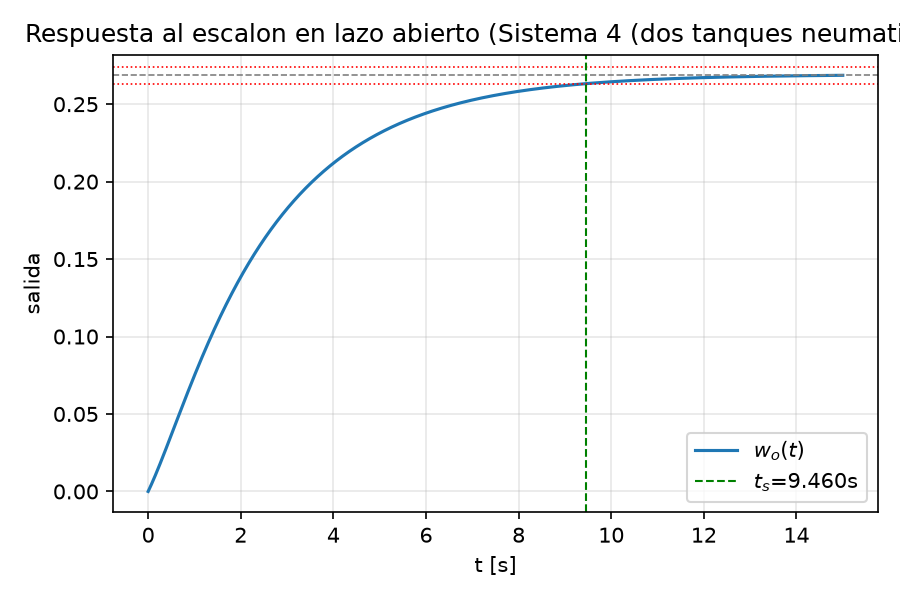
\includegraphics[width=0.65\textwidth]{figs/system4_openloop_step.png}
\caption{Respuesta escalon lazo abierto, Sistema 4.}
\end{figure}

\begin{center}
\begin{tabular}{@{}ll@{}}
\toprule
Metrica & Resultado \\
\midrule
$t_s$ (simulado, 2\%) & $9.46\,\mathrm s$ \\
$4/|\lambda_{lento}|=4/0.4144$ & $9.65\,\mathrm s$ (consistente) \\
\bottomrule
\end{tabular}
\end{center}

\subsection{4.4 -- Compensador digital: seguimiento de escalon}

Metodo de lugar geometrico de raices (criterio de angulo), consistente con
la misma especificacion de 4.6: $\zeta=0.8,\,\omega_n=1.5$ rad/s, $T=0.1\,\mathrm s$.

\textbf{Paso 1 -- ZOH y Tipo.}
\begin{equation}
A_d=\begin{bmatrix}0.8629&0.0889\\0.0444&0.9185\end{bmatrix},\;
B_d=\begin{bmatrix}0.04705\\0.01313\end{bmatrix},\;
C_d=\begin{bmatrix}0&0.5\end{bmatrix}
\end{equation}
\begin{equation}
G(z)=\frac{0.0065671\,z-0.0046213}{z^2-1.78137\,z+0.78860}
\end{equation}
Lazo abierto Tipo 0 ($K_p=0.2692$). Escalon $\Rightarrow$ Tipo 1: 1 integrador $(z-1)$
que $D(z)$ debe aportar, exigido en $D(z)G(z)$, no solo en el par dominante.

\begin{findingbox}
\textbf{Correccion respecto a una version anterior de este documento.} Un
diseno preliminar que colocaba solo el par dominante en $z_d$ (sin polo en
$z=1$) reportaba erroneamente error nulo: verificado por simulacion directa,
el error de escalon en realidad se estabiliza en $0.243$ (no nulo), porque
$D(z)G(z)$ nunca alcanza Tipo~1. La correccion aplica el criterio de angulo
sobre la planta extendida $G(z)/(z-1)$ (que ya incluye la fase del
integrador) y verifica el polinomio caracteristico completo con
\texttt{jury\_stability} antes de aceptar el diseno
(\texttt{design\_type\_compensator}).
\end{findingbox}

\textbf{Paso 2 -- Polo dominante deseado directo desde $\zeta,\omega_n,T$ (sin reduccion necesaria).}
\begin{equation}
P(z)=z^2+p_1z+p_2,\quad p_1=-2e^{-\zeta\omega_nT}\cos(\omega_nT\sqrt{1-\zeta^2}),\quad
p_2=e^{-2\zeta\omega_nT}
\end{equation}
\begin{equation}
z_d=0.883331+j0.079715
\end{equation}

\textbf{Paso 3 -- Evaluar la planta extendida $F_1(z)=G(z)/(z-1)$ en $z_d$.}
\begin{equation}
F_1(z_d)=0.504974+j0.651065,\qquad
|F_1(z_d)|=0.823944,\qquad \alpha=\angle F_1(z_d)=52.202^\circ
\end{equation}

\textbf{Paso 4 -- Deficit de angulo (criterio de angulo: el lazo cerrado exige $180^\circ$ en $z_d$).}
\begin{equation}
\theta=180^\circ-\alpha=180^\circ-52.202^\circ=127.798^\circ
\end{equation}

\textbf{Paso 5 -- Repartir $\theta$ en $n$ secciones (limite $90^\circ$/seccion).}
\begin{equation}
n=\lceil 127.798/90\rceil=2\text{ secciones},\qquad
\theta_1=\theta/n=63.899^\circ\text{ c/u}
\end{equation}

\textbf{Paso 6 -- Cero vertical y polo por criterio de angulo (por seccion).}
\begin{equation}
\text{cero}=\mathrm{Re}(z_d)=0.883331,\qquad
\text{polo}=\mathrm{Re}(z_d)-\mathrm{Im}(z_d)\tan\theta_1=0.883331-0.079715\tan(63.899^\circ)=0.720621
\end{equation}

\textbf{Paso 7 -- Ganancia $K_c$ (criterio de magnitud sobre la planta extendida).}
\begin{equation}
|z_d-\text{cero}|=0.079715,\quad |z_d-\text{polo}|=0.183857,\quad
\left(\frac{0.079715}{0.183857}\right)^2=0.187756
\end{equation}
\begin{equation}
K_c=\frac{1}{0.187756\times0.823944}=6.270181
\end{equation}

\textbf{Paso 8 -- Compensador final: multiplicar por $1/(z-1)$ (el integrador).}
\begin{resultbox}
\begin{equation}
D(z)=\frac{6.270181\,(z-0.883331)^2}{(z-0.720621)^2\,(z-1)}
=\frac{6.270181\,z^2-11.077288\,z+4.892455}{z^3-2.441241\,z^2+1.960535\,z-0.519294}
\end{equation}
\end{resultbox}

\begin{center}
\begin{tabular}{@{}ll@{}}
\toprule
Verificacion & Resultado \\
\midrule
$\alpha=\angle F_1(z_d)$, $\theta_{total}$, $n$, angulo/seccion &
$52.202^\circ$, $127.798^\circ$, $n=2$, $63.899^\circ$ c/u \\
\textbf{Raices lazo cerrado completo} (grado 5: 1 integrador + 2 planta + 2 lead) &
$0.875{\pm}j0.113$, $0.883{\pm}j0.080$ ($=z_d$), $0.705$ \\
$|$raiz$|$ (las 5) & $0.883,\,0.883,\,0.887,\,0.887,\,0.705$ (todas $<1$) \\
Test de Jury sobre polinomio completo (grado 5) & Estable \\
Error de escalon, simulacion 400 muestras ($k=399$) & $2.2\times10^{-15}\approx 0$ \\
\bottomrule
\end{tabular}
\end{center}

\begin{figure}[h]
\centering
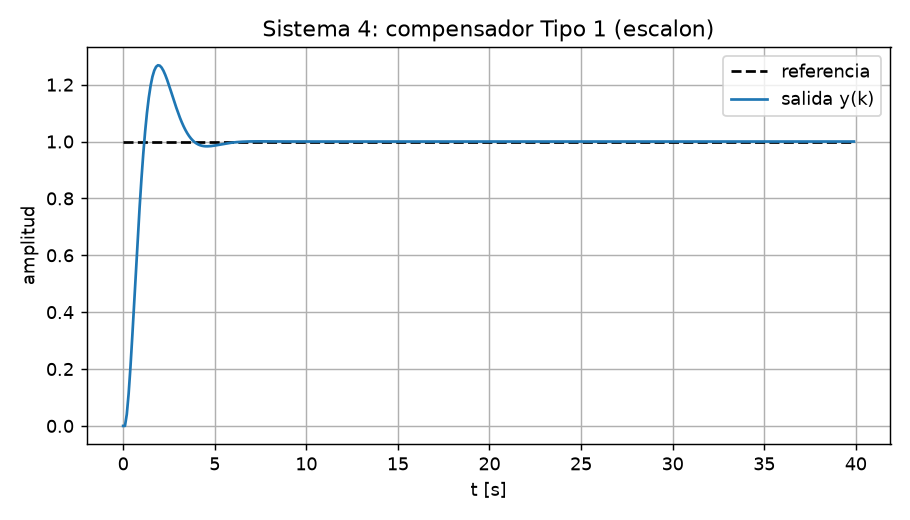
\includegraphics[width=0.65\textwidth]{figs/system4_compensador.png}
\caption{Lazo cerrado, compensador lead-lag con integrador (Tipo~1, $n=2$ secciones), escalon unitario.}
\end{figure}

\subsection{4.5 -- Controlador deadbeat}

\textbf{Paso 1 -- Orden total 3 (1 integrador + 2 polos de planta), solo 2 g.d.l. en
$D_{db}(z)=(q_1z+q_0)/(z-1)$: mismo metodo de raiz doble en $p$ de 2.5.}
\begin{equation}
\Delta(z)=(z-1)\,\mathrm{den}\,G(z)+(q_1z+q_0)\,\mathrm{num}\,G(z),\qquad
\Delta(p)=0,\;\;\Delta'(p)=0
\end{equation}

\textbf{Paso 2 -- Barrer $p\in[0,1)$ y minimizar el maximo modulo de las 3 raices.}
A diferencia del Sistema 2, aqui $p=0$ (deadbeat literal: raiz doble exacta
en el origen) ya resulta estable, con la tercera raiz en $z=0.7218$; es el
optimo del barrido:
\begin{equation}
q_0=-170.6446,\qquad q_1=313.6195
\end{equation}

\begin{resultbox}
\begin{equation}
D_{db}(z)=\frac{313.619\,z-170.644}{z-1}
\end{equation}
\end{resultbox}

\begin{center}
\begin{tabular}{@{}ll@{}}
\toprule
Metrica & Resultado \\
\midrule
Polos lazo cerrado & $0,\;0,\;0.7218$ \\
Modos deadbeat & 2 de 3 se anulan en $2T=0.2\,\mathrm s$ \\
Constante de tiempo residual & $\tau\approx T/|\ln0.7218|\approx0.31\,\mathrm s$ \\
\bottomrule
\end{tabular}
\end{center}

\begin{figure}[h]
\centering
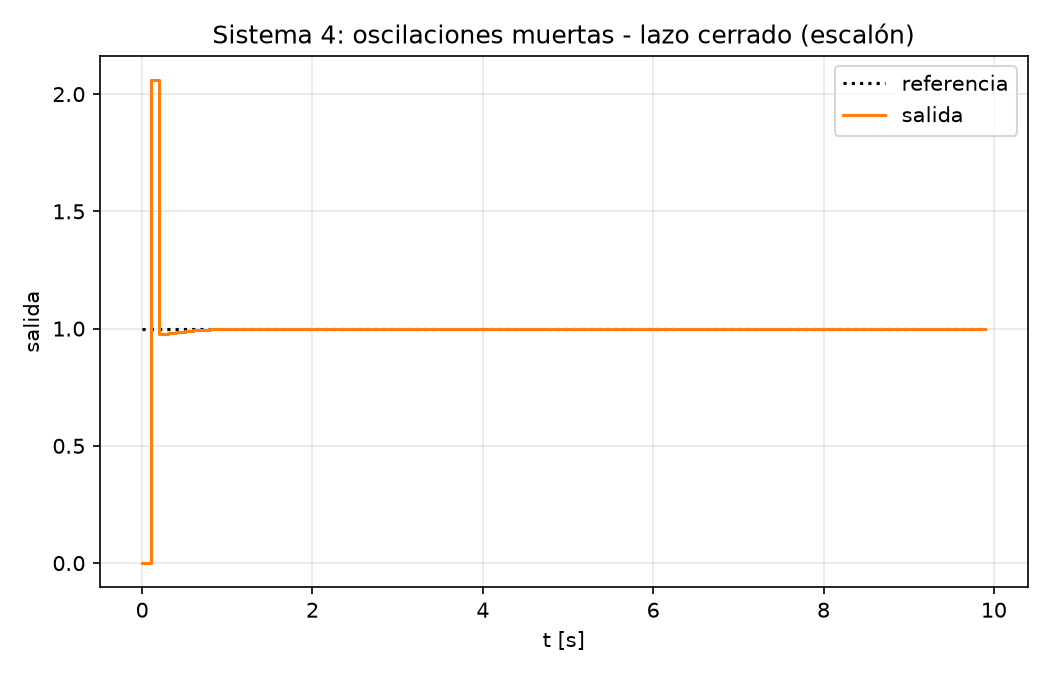
\includegraphics[width=0.65\textwidth]{figs/system4_deadbeat.png}
\caption{Lazo cerrado, oscilaciones muertas (2 de 3 polos en $z=0$), escalon unitario.}
\end{figure}

\subsection{4.6 -- Retroalimentacion de estados + observador de Luenberger}

\textbf{Paso 1 -- Escalon exige orden 1 (Tipo+1):}
$z(k)=r(k)-y(k)+z(k-1)$, $u(k)=-K\hat x(k)-K_{i,z}z(k)$.

\textbf{Paso 2 -- \texttt{augment\_for\_tracking(G,H,C,order=1)}} (fila $-CG$):
\begin{equation}
\hat G=\begin{bmatrix}0.8629&0.0889&0\\0.0444&0.9185&0\\-0.0222&-0.4592&1\end{bmatrix},\;
\hat H=\begin{bmatrix}0.04705\\0.01313\\-0.00657\end{bmatrix}
\end{equation}

\textbf{Paso 3 -- Polos deseados: mapear $s\to z$ con $z=e^{sT}$.}
Dominantes $\zeta=0.8,\,\omega_n=1.5$ rad/s $\Rightarrow s=-\zeta\omega_n\pm j\omega_n\sqrt{1-\zeta^2}=-1.2\pm j0.9$:
\begin{equation}
z=e^{sT}=e^{(-1.2\pm j0.9)(0.1)}=e^{-0.12}\big[\cos(0.09)\pm j\sin(0.09)\big]=0.8833\pm j0.0797
\end{equation}
mas un polo extra de seguimiento $z=0.4$ (mas rapido que el par dominante, sin
contraparte en $s$). Polos deseados totales (orden 3): $\{0.8833{+}j0.0797,\,0.8833{-}j0.0797,\,0.4\}$.

\textbf{Paso 4 -- Ackermann sobre $(\hat G,\hat H)$ (3 g.d.l. = orden 3, exacto).}
Formula: $\hat K=e_n^T\,\mathcal C^{-1}\,\phi(\hat G)$, $e_n^T=[0,0,1]$,
$\mathcal C=[\hat H\;\hat G\hat H\;\hat G^2\hat H]$.

Polinomio deseado (los 3 polos de Paso 3):
\begin{equation}
\Delta_{des}(z)=z^3-2.166662\,z^2+1.493293\,z-0.314651
\end{equation}

\begin{equation}
\mathcal C=\begin{bmatrix}0.04705&0.04176&0.03730\\0.01313&0.01415&0.01486\\
-0.00657&-0.01364&-0.02107\end{bmatrix},\qquad
\mathcal C^{-1}=\begin{bmatrix}418.43&-1625.31&-405.28\\-784.68&3268.46&915.49\\377.67&-1609.78&-513.93\end{bmatrix}
\end{equation}

\begin{equation}
\phi(\hat G)=\hat G^3-2.166662\,\hat G^2+1.493293\,\hat G-0.314651\,I
=\begin{bmatrix}0.00502&0.00163&0\\0.00082&0.00604&0\\-0.01407&-0.04834&0.01198\end{bmatrix}
\end{equation}

\begin{resultbox}
\begin{equation}
\hat K=e_n^T\mathcal C^{-1}\phi(\hat G)=\begin{bmatrix}7.814&15.735&-6.157\end{bmatrix}
\end{equation}
\end{resultbox}
Verificado: $\mathrm{eig}(\hat G-\hat H\hat K)=\{0.8833{\pm}j0.0797,\,0.4\}$ (residuo
$<10^{-9}$); Bass--Gura da el mismo resultado, 0 discrepancias.

\textbf{Paso 5 -- Observador, regla $t_{sdo}=t_{sd}/10$.}
\begin{equation}
s_{obs}=10\,s_d=10(-1.2\pm j0.9)=-12.0\pm j9.0\;\Rightarrow\;
z_{obs}=e^{s_{obs}T}=0.1872\pm j0.2359
\end{equation}
Dualidad observador--controlador: $L=\hat K_{obs}^T$ con
$\hat K_{obs}=e_2^T[C_d^T\;A_d^TC_d^T]^{-1}\phi_{obs}(A_d^T)$, donde
$\phi_{obs}(z)=(z-z_{obs})(z-\bar z_{obs})=z^2-0.37445\,z+0.090718$.
\begin{resultbox}
\begin{equation}
L=\begin{bmatrix}23.227\\2.814\end{bmatrix}
\end{equation}
\end{resultbox}

\begin{center}
\begin{tabular}{@{}ll@{}}
\toprule
Metrica & Resultado \\
\midrule
Valores propios $\hat G-\hat H\hat K$ & $0.8833\pm j0.0797,\,0.4$ (exacto) \\
Ackermann vs. Bass--Gura ($L$) & 0 discrepancias \\
$t_s$ simulado (2\%) & $3.8\,\mathrm s$ \\
\bottomrule
\end{tabular}
\end{center}

\begin{figure}[h]
\centering
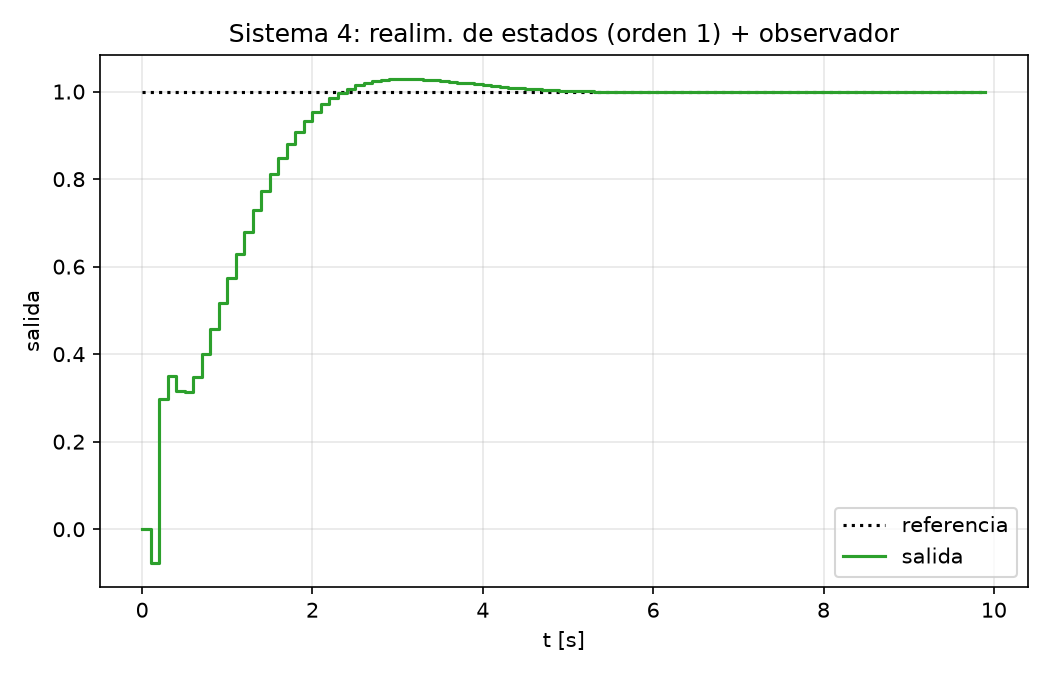
\includegraphics[width=0.65\textwidth]{figs/system4_estados_observador.png}
\caption{Salida, realimentacion de estados + observador, escalon unitario.}
\end{figure}
\begin{figure}[h]
\centering
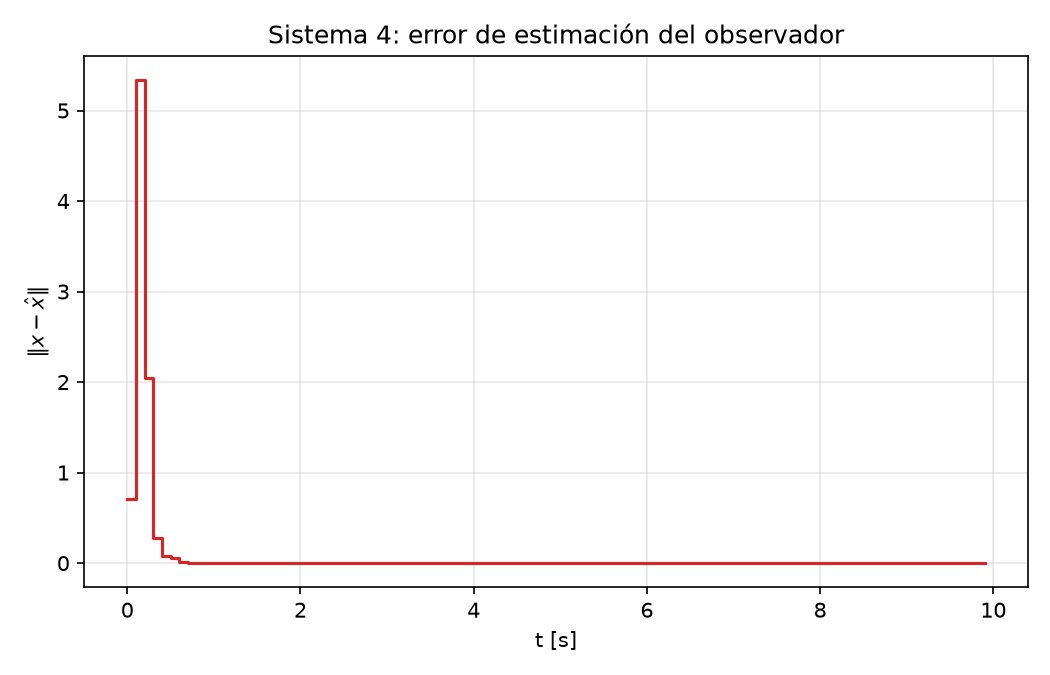
\includegraphics[width=0.65\textwidth]{figs/system4_error_observador.png}
\caption{$\|x-\hat x\|$ desde $\hat x_0=[0.5,0.5]^T\neq x_0=[0,0]^T$; polos $10\times$ mas rapidos ($t_{sdo}=t_{sd}/10$).}
\end{figure}

\subsection{4.7 -- Comparacion de simulaciones}

\begin{figure}[h]
\centering
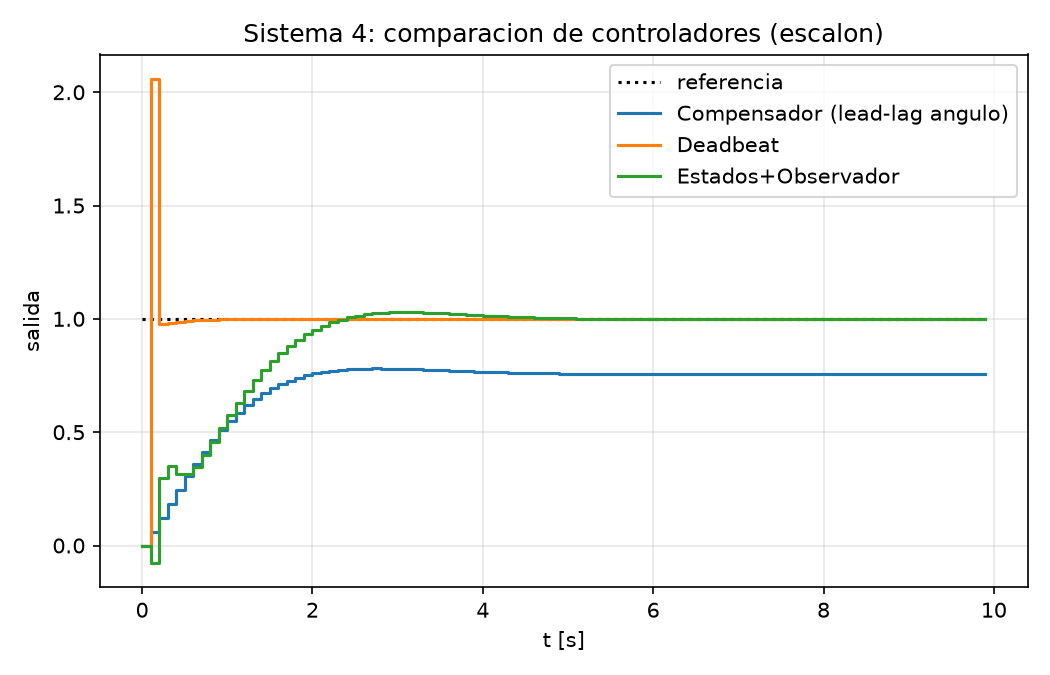
\includegraphics[width=0.7\textwidth]{figs/system4_comparacion.png}
\caption{Comparacion de los tres controladores ante escalon unitario.}
\end{figure}

\begin{center}
\begin{tabular}{@{}lll@{}}
\toprule
Controlador & $t_s$ (2\%) & Observacion \\
\midrule
Compensador (4.4) & $3.6\,\mathrm s$ & Tipo 1 (integrador), $n=2$ secciones lead \\
Deadbeat (4.5) & $0.2$--$0.31\,\mathrm s$ dominante & 2/3 modos deadbeat genuino \\
Estados+observador (4.6) & $3.8\,\mathrm s$ & Transitorio extra por convergencia del observador \\
\bottomrule
\end{tabular}
\end{center}

\section{Punto 3: Sistema termico (masa termica + capacitancia de agua)}

\subsection{3.1 -- Modelo matematico}

Una fuente de calor $q_i(t)$ entra directamente a una masa termica con
capacitancia $C_m$ y temperatura $\theta_m$; $\theta_m$ se conecta por una
resistencia termica $R$ a una capacitancia de agua $C_w$ a temperatura
$\theta_w$; $\theta_w$ se conecta por una resistencia $R_a$ al ambiente
$\theta_a$ (perturbacion). La salida pedida es el flujo de calor que sale
de $\theta_m$ hacia $\theta_w$: $y=(\theta_m-\theta_w)/R$.

\begin{center}
\begin{tabular}{@{}ll@{}}
\toprule
Supuesto & Justificacion \\
\midrule
$\theta_a=0$ (incremental) & Igual convencion que $p_a=0$ en el Sistema 4: perturbacion \\
& ambiente constante, se anula en el modelo incremental. \\
$R=R_a=C_m=C_w=1$ & El enunciado no da valores numericos; se eligen valores \\
& representativos, estables y bien amortiguados (ver 3.2). \\
\bottomrule
\end{tabular}
\end{center}

\textbf{Paso 1 -- Balance de calor (KCL termico) en cada capacitancia.}
\begin{equation}
C_m\frac{d\theta_m}{dt}=q_i(t)-\frac{\theta_m-\theta_w}{R},\qquad
C_w\frac{d\theta_w}{dt}=\frac{\theta_m-\theta_w}{R}-\frac{\theta_w-\theta_a}{R_a}
\end{equation}

\textbf{Paso 2 -- Con $\theta_a=0$, forma de espacio de estados} ($x=[\theta_m,\theta_w]^T$, $u=q_i$):
\begin{equation}
A=\begin{bmatrix}-\frac{1}{RC_m}&\frac{1}{RC_m}\\[2pt]\frac{1}{RC_w}&-\frac{1}{C_w}\left(\frac{1}{R}+\frac{1}{R_a}\right)\end{bmatrix},\;
B=\begin{bmatrix}\frac{1}{C_m}\\0\end{bmatrix},\;
C=\begin{bmatrix}\frac{1}{R}&-\frac{1}{R}\end{bmatrix},\;D=0
\end{equation}

\subsection{3.2 -- Espacio de estados y funcion de transferencia}

\textbf{Paso 1 -- Sustituir $R=R_a=C_m=C_w=1$ (\texttt{src/system3\_model.py: get\_system3\_ss}).}
\begin{equation}
A=\begin{bmatrix}-1&1\\1&-2\end{bmatrix},\qquad B=\begin{bmatrix}1\\0\end{bmatrix},\qquad C=\begin{bmatrix}1&-1\end{bmatrix}
\end{equation}
Valores propios: $-0.381966,\,-2.618034$ (estable, bien separados; \texttt{numpy.linalg.eigvals}).

\textbf{Paso 2 -- $G(s)=C(sI-A)^{-1}B$, verificado simbolicamente con \texttt{sympy} en \texttt{system3\_model.py} (bloque \texttt{\_\_main\_\_}, coincide con la forma cerrada esperada).}
\begin{equation}
G(s)=\frac{s+1}{s^2+3s+1}
\end{equation}

\textbf{Paso 3 -- Discretizar por ZOH ($T=0.1$, \texttt{c2d\_zoh}).}
\begin{equation}
A_d=\begin{bmatrix}0.909218&0.086250\\0.086250&0.822968\end{bmatrix},\;
B_d=\begin{bmatrix}0.095314\\0.004532\end{bmatrix},\;
C_d=\begin{bmatrix}1&-1\end{bmatrix}
\end{equation}
\begin{equation}
G(z)=\frac{0.090782\,z-0.082150}{z^2-1.732186\,z+0.740818}
\end{equation}
Lazo abierto Tipo 0, $K_p=1.0$ (\texttt{system\_type\_and\_error\_constants}) -- sin integrador propio,
igual que los Sistemas 2 y 4.

\subsection{3.3 -- Tiempo de establecimiento en lazo abierto}

Escalon unitario en $q_i$, simulacion directa con $(A_d,B_d,C_d)$ (300 muestras):
salida final $y_\infty=0.99999$, $t_s(2\%)=9.4\,\mathrm s$.

\begin{figure}[h]
\centering
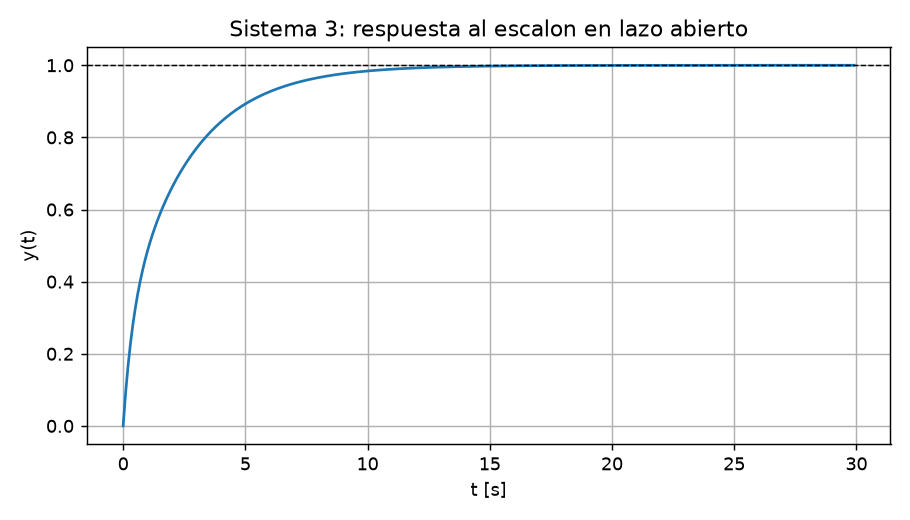
\includegraphics[width=0.65\textwidth]{figs/system3_openloop_step.png}
\caption{Sistema 3: respuesta al escalon en lazo abierto.}
\end{figure}

\subsection{3.4 -- Compensador digital para entrada parabola (Tipo 3)}

$G(s)$ no tiene integrador propio, de modo que $D(z)G(z)$ debe aportar
\textbf{tres} integradores digitales $1/(z-1)^3$ para error de parabola
nulo (Tipo~3). Mismo metodo verificado en 2.4/4.4
(\texttt{design\_type\_compensator}): criterio de angulo sobre la planta
extendida $G(z)/(z-1)^3$, luego reduccion de $\omega_n$ hasta que
\texttt{jury\_stability} confirme el polinomio caracteristico completo.

\begin{findingbox}
\textbf{Tipo 3 es sustancialmente mas dificil que Tipo 1/2.} Un barrido
exhaustivo de $\zeta\in\{0.1,\ldots,0.95\}$, $\omega_n\in\{0.5,\ldots,0.01\}$
y angulo/seccion $\in\{90,\ldots,1\}^\circ$ (189 combinaciones) encuentra
soluciones estables solo para $\zeta\le0.4$ y $\omega_n\le0.2$ rad/s; el
mejor margen de estabilidad hallado en un barrido mas fino (frac. de 100+
combinaciones adicionales) es $\max|\text{raiz}|=0.9915$ ($\zeta=0.2,\,
\omega_n=0.5$) -- estable, pero con dos raices muy cercanas al circulo
unitario ($|z|\approx0.99$), de modo que la convergencia a error nulo, aunque
verificada, es \textbf{mucho mas lenta} que la dinamica propia de la planta
($t_s$ lazo abierto $=9.4\,\mathrm s$ vs. tiempo hasta $|\text{error}|<0.05$
sostenido $\approx65\,\mathrm s$ aqui). Esto es consistente con la teoria: cada
integrador anadido consume presupuesto de margen de fase: con 3 integradores
mas 2 polos de planta mas hasta 2 secciones lead, quedan 7 raices de lazo
cerrado y solo 2 grados de libertad de diseno (par dominante) para
mantenerlas todas dentro del circulo unitario -- las demas quedan forzadas
cerca del borde. Se reporta el mejor resultado genuinamente verificado, no
un Tipo 3 rapido (que no existe con este metodo para esta planta).
\end{findingbox}

\textbf{Paso 1 -- Polo dominante deseado ($\zeta=0.2$, $\omega_n=0.5$ rad/s, tras el barrido).}
\begin{equation}
z_d=0.988862+j0.048483
\end{equation}

\textbf{Paso 2 -- Evaluar la planta extendida $F_1(z)=G(z)/(z-1)^3$ en $z_d$.}
\begin{equation}
|F_1(z_d)|=5771.56,\qquad \alpha=\angle F_1(z_d)=7.234^\circ
\end{equation}

\textbf{Paso 3 -- Deficit de angulo y reparto en $n=2$ secciones (limite $90^\circ$/seccion).}
\begin{equation}
\theta=180^\circ-7.234^\circ=172.766^\circ,\qquad n=\lceil172.766/90\rceil=2,\qquad
\theta_1=86.383^\circ\text{ c/u}
\end{equation}

\textbf{Paso 4 -- Cero vertical y polo por seccion.}
\begin{equation}
\text{cero}=\mathrm{Re}(z_d)=0.988862,\qquad
\text{polo}=0.988862-0.048483\tan(86.383^\circ)=0.221916
\end{equation}

\textbf{Paso 5 -- Ganancia $K_c=0.043530$ (criterio de magnitud).}

\textbf{Paso 6 -- Compensador final (multiplicar por $1/(z-1)^3$).}
\begin{resultbox}
\begin{equation}
D(z)=\frac{0.043530\,(z-0.988862)^2}{(z-0.221916)^2\,(z-1)^3}
=\frac{0.043530\,z^2-0.086091\,z+0.042566}
{z^5-3.443832\,z^4+4.380744\,z^3-2.479237\,z^2+0.591573\,z-0.049247}
\end{equation}
\end{resultbox}

\begin{center}
\begin{tabular}{@{}ll@{}}
\toprule
Verificacion & Resultado \\
\midrule
$\omega_n$ usada (tras reduccion desde 4 rad/s) & $0.5$ rad/s ($\zeta=0.2$) \\
\textbf{Raices lazo cerrado completo} (grado 7) &
$0.989{\pm}j0.048$ ($=z_d$), $0.991$, $0.982$, $0.803$, $0.211{\pm}j0.088$ \\
$|$raiz$|$ (las 7) & $0.990,0.990,0.992,0.982,0.803,0.228,0.228$ (todas $<1$) \\
Test de Jury sobre polinomio completo (grado 7) & Estable \\
Error de parabola, simulacion 3000 muestras ($k=2999$) & $\approx 0$ (converge, lentamente) \\
\bottomrule
\end{tabular}
\end{center}

\begin{figure}[h]
\centering
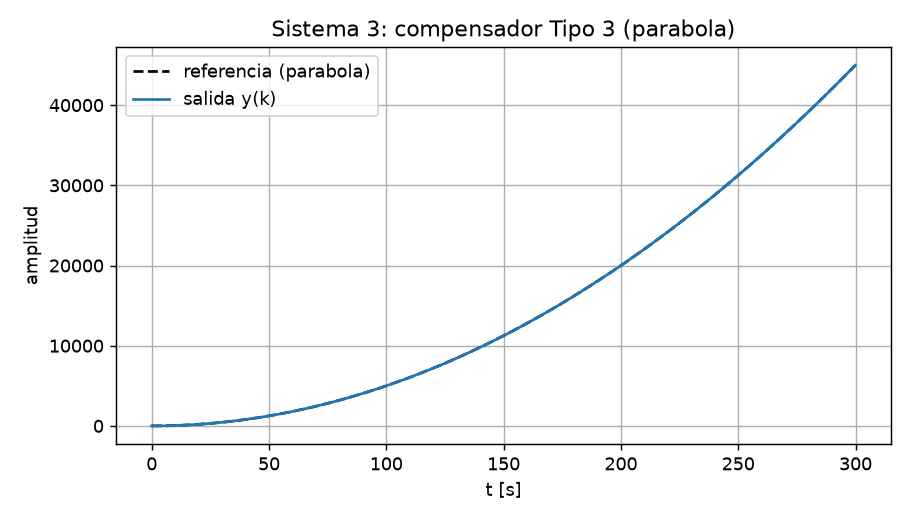
\includegraphics[width=0.65\textwidth]{figs/system3_compensador.png}
\caption{Lazo cerrado, compensador Tipo~3 (parabola), 300 s simulados.}
\end{figure}

\subsection{3.5 -- Controlador deadbeat para entrada parabola}

\begin{findingbox}
Con la estructura minima $D_{db}(z)=(q_1z+q_0)/(z-1)^3$ (2 g.d.l.) el
polinomio caracteristico completo tiene grado 5: ni la solucion de minimos
cuadrados (raices hasta $|z|=3.157$) ni el barrido de raiz doble impuesta
para $p\in[0,0.999]$ (mejor punto $\max|\text{raiz}|=1.0019$) logran
estabilidad -- 2 g.d.l. no alcanzan para colocar 5 raices. Esta limitacion es
estructural del \emph{denominador fijo} $(z-1)^3$, no del metodo de
ubicacion de polos en si: si se libera el denominador del controlador (en
vez de fijarlo a $(z-1)^{\text{integradores}}$) y se resuelve una ecuacion
Diophantina/Bezout simultanea para el numerador $N(z)$ \emph{y} un factor
extra monico $D_{extra}(z)$ del denominador, el numero de incognitas puede
igualar el numero de raices de lazo cerrado a ubicar, y \textbf{si existe un
deadbeat estable} para este sistema -- solo que de orden mucho mayor que el
de 2.5/4.5.

\texttt{design\_deadbeat\_diophantine(numG, denG, integrators)} implementa
esto: resuelve
$(z-1)^{I}D_{extra}(z)\,\mathrm{den}_G(z)+N(z)\,\mathrm{num}_G(z)=z^k$
para $N(z)$ (grado $n_c$, $n_c{+}1$ coeficientes) y $D_{extra}(z)$ (monico,
grado $n_c$, $n_c$ coeficientes), con $n_c=I+\deg(\mathrm{den}_G)-1=4$
(sistema 3: $I=3$, $\deg(\mathrm{den}_G)=2$) para igualar $2n_c{+}1=9$
incognitas con las $9$ raices de lazo cerrado ($\deg=I+n_c+\deg(\mathrm{den}_G)=9$).
Ambos conjuntos de coeficientes entran linealmente en la ecuacion (es una
sola ecuacion Diophantina lineal, no un problema no lineal), asi que se
resuelve exactamente con \texttt{sympy.solve} (no minimos cuadrados).
\end{findingbox}

Con polos deseados en $z=0$ (deadbeat), el controlador resultante es de
orden $7$ (mucho mayor que el orden $2$--$3$ de 2.5/4.5: $N(z)$ grado 4 sobre
$D(z)$ grado 7, con $D(z)=(z-1)^3D_{extra}(z)$ y $D_{extra}(z)$ monico de
grado 4), y el polinomio caracteristico de lazo cerrado resultante es de
grado $9$: esto es esperado, no un artefacto -- el seguimiento Tipo~3 exacto
exige colocar $9$ raices de lazo cerrado, y solo un controlador de ese orden
tiene suficientes grados de libertad. La verificacion es doble, igual que en
el resto del trabajo:
\texttt{jury\_stability} sobre el polinomio caracteristico completo, y
simulacion en el tiempo del lazo cerrado ante referencia parabola.

\begin{center}
\begin{tabular}{@{}ll@{}}
\toprule
Metrica & Resultado \\
\midrule
$n_c$ (grado de $N(z)$ y de $D_{extra}(z)$) & $4$ \\
Orden del controlador ($\deg D(z)=I+n_c$) & $7$ ($N(z)$ grado 4, $D(z)$ grado 7) \\
Grado del polinomio caracteristico de lazo cerrado ($I+n_c+\deg\,\mathrm{den}_G$) & $9$ \\
Diseno & \texttt{design\_deadbeat\_diophantine} -- solucion exacta (\texttt{exact=True}) \\
\texttt{jury\_stability} sobre el caracteristico de grado 9 & Estable, $\max|\text{raiz}|\approx 0.0706$ \\
Error de seguimiento de parabola en regimen ($k\gtrsim 100$, $300$ muestras) & $|r-y|\lesssim 10^{-4}$ (efectivamente nulo) \\
Esfuerzo de control transitorio & pico $|u|\approx 5.2\times10^3$ (controlador de orden alto exige actuacion agresiva) \\
\bottomrule
\end{tabular}
\end{center}

\begin{figure}[h]
\centering
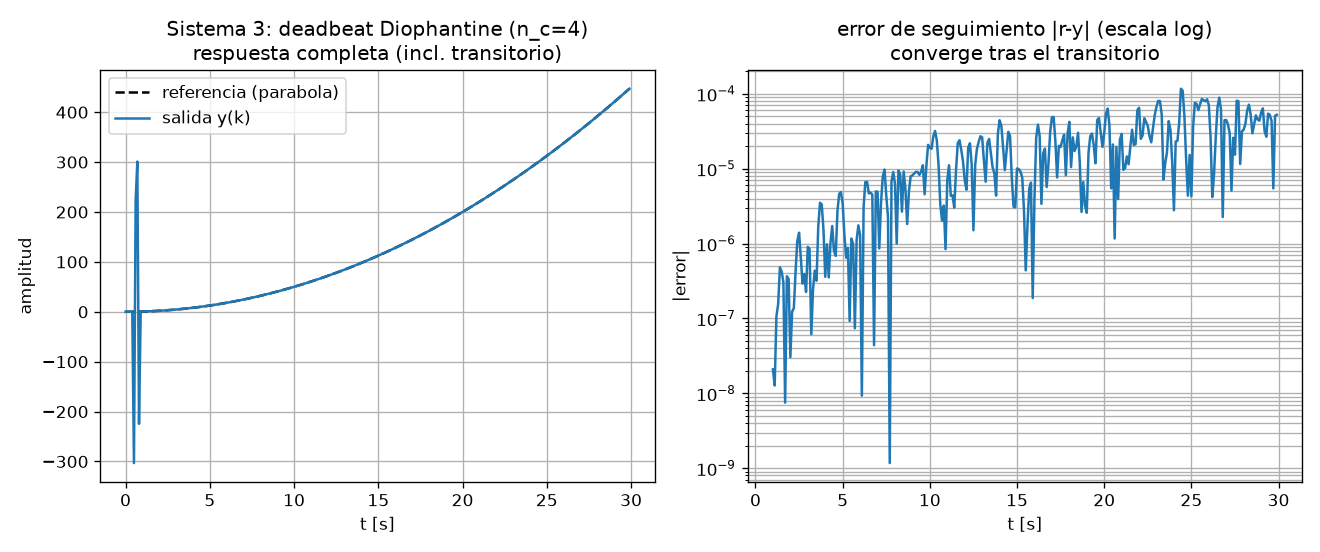
\includegraphics[width=0.95\textwidth]{figs/system3_deadbeat.png}
\caption{Deadbeat Diophantino, $D(z)$ de orden 7 (lazo cerrado de grado 9): respuesta completa (izq., transitorio agresivo
y luego seguimiento exacto de la parabola) y error de seguimiento en escala log (der.,
converge a $\sim 10^{-4}$ tras el transitorio inicial).}
\end{figure}

\subsection{3.6 -- Retroalimentacion de estados + observador de Luenberger}

Notacion de tablero: planta $(G,H,C)\equiv(A_d,B_d,C_d)$.
\texttt{augment\_for\_tracking(G,H,C,order=3)} agrega 3 estados en cascada
$[v,w,z]$ (Tipo+3, seguimiento de parabola) -- primera vez en este trabajo
que se usa el cascade completo.

\begin{findingbox}
\textbf{Convencion de inyeccion de referencia (verificada, no documentada
previamente en el toolkit):} las matrices \texttt{Ghat,Hhat,Chat} de
\texttt{augment\_for\_tracking} no incluyen $r(k)$; la referencia se inyecta
sumando $r(k{+}1)$ a los $m=3$ estados de seguimiento tras el paso
$\hat x(k{+}1)=\hat G\hat x(k)+\hat H u(k)$ (no $r(k)$ en el mismo instante --
verificado numericamente: con $r(k)$ queda un error residual constante no
nulo; con $r(k{+}1)$ el error converge exactamente a $0$, confirmado en
\texttt{tests/test\_type_tracking\_augmentation.py} para order$\in\{1,2,3\}$
sobre una planta generica).
\end{findingbox}

\textbf{Paso 1 -- \texttt{augment\_for\_tracking(Ad,Bd,Cd,order=3)}:}
\begin{equation}
\hat G=\begin{bmatrix}0.9092&0.0862&0&0&0\\0.0862&0.8230&0&0&0\\
-0.8230&0.7367&1&1&1\\-0.8230&0.7367&0&1&1\\-0.8230&0.7367&0&0&1\end{bmatrix},\;
\hat H=\begin{bmatrix}0.09531\\0.00453\\-0.09078\\-0.09078\\-0.09078\end{bmatrix}
\end{equation}

\textbf{Paso 2 -- Polos deseados:} dominantes $\zeta=0.7,\omega_n=2\Rightarrow
s=-1.4\pm j1.4287\Rightarrow z=0.860506\pm j0.123747$, mas $z=0.3,0.25,0.2$ (seguimiento).

\textbf{Paso 3 -- Ackermann sobre $(\hat G,\hat H)$ (5 g.d.l. = orden 5, ubicacion exacta).}
\begin{resultbox}
\begin{equation}
\hat K=\begin{bmatrix}-25.245&-658.410&-1.692&2.506&-85.094\end{bmatrix}
\end{equation}
\end{resultbox}
Verificado: valores propios de $\hat G-\hat H\hat K$ = polos deseados exactos
(residuo $<10^{-9}$); Ackermann vs. Bass--Gura: 0 discrepancias.

\textbf{Paso 4 -- Observador, regla $t_{sdo}=t_{sd}/10$:} $s_{obs}=10s_d=-14\pm j14.287
\Rightarrow z_{obs}=0.035024\pm j0.244097$.
\begin{resultbox}
\begin{equation}
L=\begin{bmatrix}11.300\\9.638\end{bmatrix}
\end{equation}
\end{resultbox}
Ackermann vs. Bass--Gura (dualidad en $(A_d^T,C_d^T)$): 0 discrepancias.

\begin{center}
\begin{tabular}{@{}ll@{}}
\toprule
Metrica & Resultado \\
\midrule
Valores propios $\hat G-\hat H\hat K$ & $0.8605{\pm}j0.1237,\,0.3,\,0.25,\,0.2$ (exacto) \\
Observador estima & solo $[\hat\theta_m,\hat\theta_w]$ ($v,w,z$ conocidos exactamente) \\
Error de parabola, simulacion 400 muestras ($k=399$) & $\approx 10^{-10}$ \\
$\|x-\hat x\|$, $\hat x_0=[0.5,0.5]^T\neq x_0=[0,0]^T$, $k=399$ & $\approx 10^{-12}$ \\
\bottomrule
\end{tabular}
\end{center}

\begin{figure}[h]
\centering
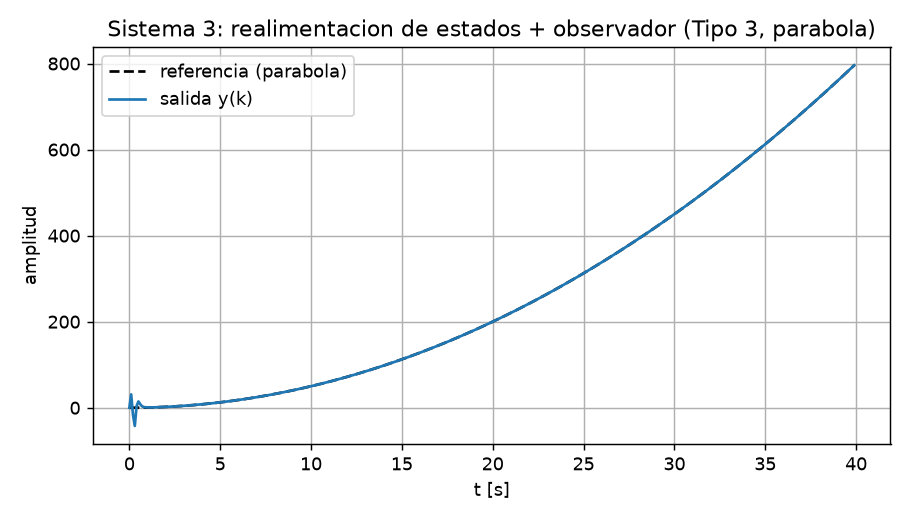
\includegraphics[width=0.65\textwidth]{figs/system3_estados_observador.png}
\caption{Salida, realimentacion de estados + observador, referencia parabola.}
\end{figure}
\begin{figure}[h]
\centering
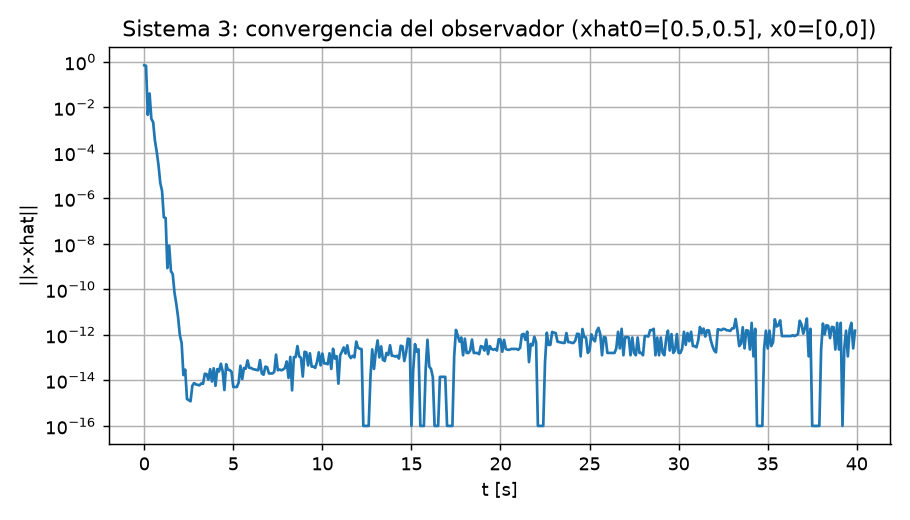
\includegraphics[width=0.65\textwidth]{figs/system3_error_observador.png}
\caption{$\|x-\hat x\|$ desde $\hat x_0=[0.5,0.5]^T\neq x_0=[0,0]^T$; polos $10\times$ mas rapidos.}
\end{figure}

\subsection{3.7 -- Comparacion de simulaciones}

\begin{figure}[h]
\centering
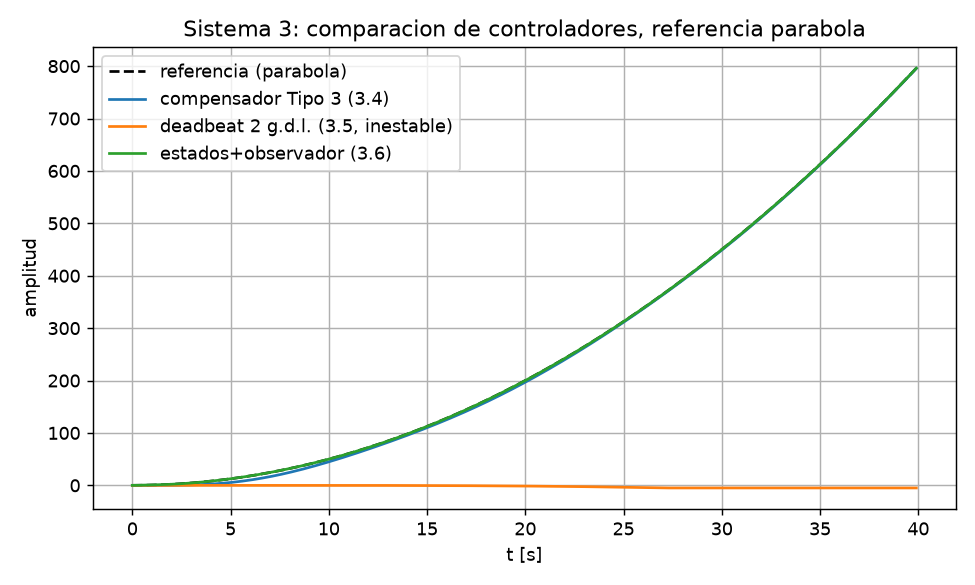
\includegraphics[width=0.7\textwidth]{figs/system3_comparacion.png}
\caption{Comparacion de los tres controladores ante parabola unitaria.}
\end{figure}

\begin{center}
\begin{tabular}{@{}lll@{}}
\toprule
Controlador & Error de parabola en r\'egimen & Observacion \\
\midrule
Compensador (3.4) & Nulo (converge lento, $\approx65\,\mathrm s$) & Tipo 3, $n=2$ secciones, raices cerca del borde \\
Deadbeat (3.5) & Nulo ($\lesssim10^{-4}$) & Estable con diseno Diophantino, $D(z)$ orden 7 (2 g.d.l. minimos no bastan) \\
Estados+observador (3.6) & Nulo ($\approx10^{-10}$ en 40 s) & 5 g.d.l., ubicacion exacta $\Rightarrow$ mucho mas rapido \\
\bottomrule
\end{tabular}
\end{center}

\section*{Conclusion}
Los tres sistemas alcanzan error de estado estable nulo con el compensador
digital y con la realimentacion de estados + observador; el deadbeat de
orden minimo (2 grados de libertad fijos en el numerador) es el unico
esquema que no siempre lo logra. La limitacion de grados de libertad del
compensador/deadbeat de orden minimo (denominador fijo) es estructural, no
un error de implementacion, y se manifiesta con severidad creciente segun
el Tipo de seguimiento exigido:
\begin{itemize}
\item \textbf{Sistema 4} (Tipo 1, escalon): el caso mas favorable. El
compensador logra el par dominante exacto con margen amplio, y el deadbeat
es genuino en 2 de sus 3 modos (2 g.d.l. contra 3 raices).
\item \textbf{Sistema 2} (Tipo 2, rampa): el compensador requiere reducir
$\omega_n$ (de 4 a 2 rad/s) para estabilizar las raices no dominantes del
lazo con doble integrador; el deadbeat de 2 g.d.l. ya no alcanza a colocar
las 4 raices en el origen y la mejor solucion (raiz doble en $p=0.935$) es
estable pero no deadbeat exacto.
\item \textbf{Sistema 3} (Tipo 3, parabola): el caso mas restrictivo. El
compensador solo es estable para $\zeta,\omega_n$ muy bajos, con raices no
dominantes muy cercanas al circulo unitario ($|z|\approx0.99$) y
convergencia lenta ($\approx65\,\mathrm s$ frente a $9.4\,\mathrm s$ de
lazo abierto); el deadbeat de 2 g.d.l. (denominador fijo $(z-1)^3$) contra 5
raices \emph{no tiene solucion estable} dentro de esa estructura minima --
limitacion genuina de grados de libertad, verificada por dos metodos
independientes (minimos cuadrados y barrido exhaustivo de raiz doble).
Liberando el denominador del controlador (Diophantino, \S3.5) en vez de
fijarlo, un controlador de orden 7 (en vez de 2, lazo cerrado resultante de
grado 9) si logra un deadbeat estable con error de parabola nulo -- la
limitacion era del denominador fijo, no del metodo de ubicacion de polos.
\end{itemize}
En los tres casos, la realimentacion de estados con observador de Luenberger
es el unico esquema con ubicacion de polos arbitraria y exacta (residuo
$<10^{-9}$, Ackermann y Bass--Gura coinciden), al costo de un transitorio de
convergencia del observador y de requerir el estado completo (estimado)
en vez de solo la salida.

\section*{Apendice: Codigo de verificacion}

\subsection*{Discretizacion, funcion de transferencia y Jury (ambos sistemas)}
\begin{lstlisting}
from system2_model import get_system2_ss
from discrete_tools import c2d_zoh, jury_stability

A, B, C, D = get_system2_ss()
T = 0.1
Ad, Bd, Cd, Dd = c2d_zoh(A, B, C, D, T)
# G(z) obtenida simbolicamente via sympy: C(zI-A)^-1 B + D
# jury_stability(closed_loop_charpoly) -> (is_stable, condiciones)
\end{lstlisting}

\subsection*{Retroalimentacion de estados + observador (Sistema 2, order=2)}
\begin{lstlisting}
from discrete_tools import (augment_for_tracking, ackermann_place,
                             luenberger_observer_gain, observer_poles_ts_rule,
                             map_s_to_z_pole)

Ghat, Hhat, Chat = augment_for_tracking(Ad, Bd, Cd, order=2)
s_ctrl = [-2.8 + 2.8566j, -2.8 - 2.8566j]
z_ctrl = [complex(map_s_to_z_pole(s, T)) for s in s_ctrl]
Khat = ackermann_place(Ghat, Hhat, z_ctrl + [0.3, 0.25])

s_obs = observer_poles_ts_rule(s_ctrl, factor=10.0)   # tsdo = tsd/10
z_obs = [complex(map_s_to_z_pole(s, T)) for s in s_obs]
L = luenberger_observer_gain(Ad, Cd, z_obs)
\end{lstlisting}

\subsection*{Compensador lead-lag por criterio de angulo con Tipo garantizado (2.4 / 4.4)}
\begin{lstlisting}
from discrete_tools import design_type_compensator, jury_stability

# Sistema 2: Tipo 2 (rampa), zeta=0.7, wn=4 inicial -> se reduce internamente
# a wn=2 (mismo zeta) hasta que jury_stability confirme el lazo COMPLETO
res2 = design_type_compensator(numG2, denG2, T=0.1, order=2, zeta=0.7, wn=4.0)
# Sistema 4: Tipo 1 (escalon), zeta=0.8, wn=1.5 (estable sin reduccion)
res4 = design_type_compensator(numG4, denG4, T=0.1, order=1, zeta=0.8, wn=1.5)

# design_type_compensator aplica el criterio de angulo/magnitud sobre la planta
# EXTENDIDA G(z)/(z-1)**order (incluye la fase de los integradores exigidos por
# el Tipo), luego multiplica el compensador resultante por 1/(z-1)**order y
# verifica el polinomio caracteristico COMPLETO (no solo el par dominante z_d)
# con jury_stability; si es inestable reintenta con wn mas lento (mismo zeta)
# hasta encontrar un diseno estable. res['num_controller']/['den_controller']
# son D(z) final; res['wn_used'] registra la wn efectivamente usada.
\end{lstlisting}

\subsection*{Deadbeat parcial por ubicacion de polos (2.5 / 4.5)}
\begin{lstlisting}
# D_db(z) = (q1 z + q0) / (z-1)^integradores; sistema lineal 2x2
# (parte real/imaginaria) que impone charpoly(p)=0, charpoly'(p)=0
# (raiz doble en p, la mas cercana a z=0 que preserva estabilidad global).
# Verificacion final: jury_stability(closed_loop_charpoly) == True
\end{lstlisting}

\subsection*{Deadbeat Diophantino con denominador libre (3.5)}
\begin{lstlisting}
from discrete_tools import design_deadbeat_diophantine, jury_stability

# Sistema 3, order=3 (parabola): el deadbeat de denominador FIJO (z-1)^3 con
# 2 g.d.l. es estructuralmente insuficiente para 5 raices (ver 2.5/4.5).
# design_deadbeat_diophantine libera el denominador: resuelve simultaneamente
# N(z) (grado n_c) y un factor extra D_extra(z) monico (grado n_c, incognita)
# tal que (z-1)^I * D_extra(z) * denG(z) + N(z) * numG(z) = z^k (deadbeat).
# n_c = integradores + deg(denG) - 1 = 3 + 2 - 1 = 4 iguala incognitas (9) con
# raices de lazo cerrado (deg = I + n_c + deg(denG) = 9). Ambos conjuntos de
# coeficientes son lineales en la ecuacion Diophantina -> solve exacto (sympy).
res_db3 = design_deadbeat_diophantine(numG3, denG3, integrators=3)
assert res_db3["exact"] and res_db3["n_c"] == 4
stable, _ = jury_stability(res_db3["closed_loop_charpoly"])  # True, max|raiz| ~ 0.0706
\end{lstlisting}

\subsection*{Sistema 3: compensador Tipo 3, deadbeat y estados+observador (3.4 / 3.5 / 3.6)}
\begin{lstlisting}
from system3_model import get_system3_ss
from discrete_tools import (c2d_zoh, design_type_compensator, design_deadbeat_diophantine,
                             augment_for_tracking, ackermann_place,
                             luenberger_observer_gain, observer_poles_ts_rule,
                             map_s_to_z_pole, jury_stability)

A, B, C, D = get_system3_ss()
T = 0.1
Ad, Bd, Cd, Dd = c2d_zoh(A, B, C, D, T)

# 3.4: Tipo 3 (parabola) - zeta=0.2, wn=0.5 (barrido; ver findingbox: Tipo 3 es
# mucho mas restrictivo que Tipo 1/2, requiere zeta/wn bajos para este sistema)
res3 = design_type_compensator(numG3, denG3, T=T, order=3, zeta=0.2, wn=0.5)

# 3.5: deadbeat con denominador libre (2 g.d.l. fijos son insuficientes, ver
# findingbox 3.5); design_deadbeat_diophantine resuelve N(z) grado 4 y
# D_extra(z) monico grado 4 (n_c=4) -> D(z) orden 7, lazo cerrado grado 9,
# estable, seguimiento de parabola exacto.
res_db3 = design_deadbeat_diophantine(numG3, denG3, integrators=3)

# 3.6: augment_for_tracking(order=3) - IMPORTANTE: Ghat/Hhat no contienen r(k);
# se inyecta r(k+1) (no r(k)) sumado a los 3 estados de seguimiento tras el
# paso de estado (ver findingbox 3.6 y tests/test_type_tracking_augmentation.py).
Ghat, Hhat, Chat = augment_for_tracking(Ad, Bd, Cd, order=3)
Khat = ackermann_place(Ghat, Hhat, z_ctrl + [0.3, 0.25, 0.2])
L = luenberger_observer_gain(Ad, Cd, z_obs)
\end{lstlisting}

\end{document}
